\documentclass[11pt,a4paper,titlepage]{article}

\title {DiaScope AI: A Web Application for Diabetes Risk Prediction with Calibrated Explainable AI using Philippine Data}
\author {James Angelo R. Dela Cruz \\ Department of Physical Sciences and Mathematics \\ University of the Philippines Manila \\ \\
Adviser: Geoffrey A. Solano}
\date{}

\usepackage[top=1in, bottom=1in, left=1.5in, right=1in]{geometry}
\usepackage{setspace}
\usepackage{amsmath}
\usepackage{url}
\usepackage{graphicx}
\usepackage{float}
\doublespacing

% allows for separate page section by changing the behavior of \section
\let\stdsection\section
\renewcommand\section{\newpage\stdsection}

\begin{document}
\maketitle
\tableofcontents

\section{Introduction}
\pagenumbering{arabic}
\setcounter{page}{1}

\subsection{Background of the Study}
Diabetes is a chronic disease characterized by elevated blood sugar levels and remains a significant public health concern in the Philippines. Individuals with diabetes face higher risks of cardiovascular disease, kidney failure, nerve damage, and vision impairment \cite{Khokhar2025}. Recent national data reveal that the prevalence of diabetes among Filipino adults has reached approximately 7.5\% as of 2024, with over 4.7 million cases reported and an alarming number of undiagnosed individuals, surpassing 53\% of the diabetes-affected population \cite{IDFPhilippines2025}. In 2020 alone, diabetes accounted for 37,265 deaths, ranking as the fourth leading cause of mortality in the country \cite{Cudis2021}. The increasing urbanization, sedentary lifestyles worsened by COVID-19 lockdowns, and changing dietary patterns have accelerated obesity and other risk factors among Filipinos, intensifying the diabetes epidemic \cite{Cando2024}.

Despite numerous international studies on diabetes risk assessment, most rely on data from Western or global populations \cite{Kiran2025}, failing to account for the unique Filipino demographic, genetic, and environmental factors \cite{Cando2024}. This reliance on international datasets undermines the applicability and reliability of predictive models for local populations, which presents a distinctive research gap. The need for a customized, locally relevant platform for accurate diabetes risk prediction is critical to improving public health outcomes \cite{Khokhar2025}. Recent advancements in artificial intelligence (AI) and machine learning have opened new avenues for medical diagnostics and predictive healthcare. However, transparency and interpretability remain major challenges for clinical adoption. Explainable Artificial Intelligence (XAI) bridges this gap by providing interpretable predictions that empower healthcare practitioners and patients alike. 

In the Philippine context, there is a pressing need for predictive models tailored to local data to ensure confidence in clinical decisions. This study addresses this need by developing a machine learning system built around four key components. The first is a comprehensive evaluation of multiple machine learning models, including tree-based algorithms and deep learning approaches trained exclusively on Philippine-specific data, to identify the optimal predictor. The second is Explainable Artificial Intelligence (XAI) techniques, specifically SHAP (SHapley Additive exPlanations) and LIME (Local Interpretable Model-agnostic Explanations), to provide interpretable explanations of model predictions at both the global and individual patient level. The third is post-hoc probability calibration methods, including Platt Scaling, Isotonic Regression, and Temperature Scaling, to align predicted risk scores with actual clinical risk levels. The fourth is Calibrated Explanations (CE) using Venn-Abers calibration, which extends standard XAI by providing each prediction with a confidence interval, generating counterfactual alternatives that suggest actionable changes to reduce a patient's risk, and conducting a sex-stratified fairness analysis to examine whether the model is equally reliable across different patient groups. By combining these components, this research aims to develop a diabetes risk prediction system that is accurate, interpretable, well-calibrated, and clinically relevant for Filipino communities.


\subsection{Statement of the Problem}
Diabetes is a significant health challenge in the Philippines, and machine learning models have shown promise in predicting its risk. While Explainable Artificial Intelligence (XAI) techniques such as SHAP and LIME help provide transparency into model predictions, they primarily offer explanations based on feature importance without indicating how confident or uncertain those explanations are for each individual patient. At the same time, probability calibration methods such as Platt Scaling and Isotonic Regression improve the reliability of predicted risk scores but do not directly communicate the uncertainty range around each prediction, nor do they suggest what a patient could change to lower their predicted risk.

This study addresses these limitations by incorporating Calibrated Explanations (CE) using the Venn-Abers calibration framework alongside SHAP, LIME, and post-hoc calibration. CE generates uncertainty-bounded explanations and counterfactual alternatives at the individual patient level, making predictions not only reliable but also actionable. The integration of these methods aims to produce a diabetes risk prediction system that is accurate, transparent, well-calibrated, and informative enough to support real clinical decision-making based on Philippine health data.

\subsection{Research Questions}

This study aims to answer the following research questions:

\begin{enumerate}
    \item Which among the evaluated machine learning models, specifically Naive Bayes, k-Nearest Neighbors, Random Forest, XGBoost, LightGBM, CatBoost, AdaBoost, Bayesian-Optimized TabNet, and ensemble methods (Voting and Stacking), achieves the best diabetes risk prediction performance on the DOST-FNRI 2018--2021 Expanded National Nutrition Survey dataset, as measured by F2-score and AUPRC?

    \item How do probability calibration techniques, specifically Platt Scaling, Isotonic Regression, and Temperature Scaling, affect the reliability of predicted diabetes risk probabilities from the best-performing model, as assessed by Brier Score, Expected Calibration Error (ECE), and calibration plots?

    \item What are the most influential clinical, anthropometric, and biochemical features driving individual diabetes risk predictions in the Philippine context, as identified by SHAP and LIME explanations applied to the best-performing calibrated model?

    \item How does Calibrated Explanations (CE) with Venn-Abers calibration characterize per-instance prediction uncertainty, and what counterfactual alternatives does it provide for at-risk individuals? Furthermore, how does model calibration quality differ between patient sex groups under a Mondrian CE framework?

    \item How can the best-performing calibrated model with XAI explanations be effectively delivered through a web-based decision support tool that provides real-time diabetes risk assessment with interpretable, probability-calibrated outputs for end-users?
\end{enumerate}

\subsection{Objectives of the Study}

The study aims to facilitate early detection and prediction of diabetes risk among individuals in the Philippines. Calibration techniques will be applied to improve the reliability of predicted probabilities, and XAI methods will be integrated to provide interpretable explanations. The specific objectives of this study are as follows:

\begin{enumerate}
    \item Allows the primary user (healthcare practitioner or end-user) to:
    \begin{enumerate}
        \item Input personal health information relevant to diabetes risk prediction (e.g., age, gender, medical history, anthropometric and biochemical measurements).
        \item Request a diabetes risk assessment that classifies whether the individual is at risk (fasting blood sugar $\geq$ 100 mg/dL) based on the input data.
        \item Receive an interpretable explanation of the prediction through XAI methods, specifically SHAP (SHapley Additive exPlanations) and LIME (Local Interpretable Model-agnostic Explanations), to help understand the key factors influencing the model's output.
        \item View the model's output in the form of a calibrated diabetes risk probability and risk level classification, including a prediction confidence interval and, where applicable, counterfactual suggestions for risk reduction, supporting informed decision-making and preventive actions.
    \end{enumerate}

    \item Allows the system to:
    \begin{enumerate}
        \item Perform comprehensive data pre-processing on the DOST-FNRI 2018--2021 ENNS dataset, including missing value imputation, target variable encoding, feature scaling (StandardScaler), correlation-based feature elimination, and class imbalance handling (SMOTE).
        \item Apply hyperparameter tuning via RandomizedSearchCV (optimizing for F2-score) to the following models: k-Nearest Neighbors, AdaBoost, XGBoost, Random Forest, LightGBM, and CatBoost, and Bayesian Optimization via Optuna for TabNet.
        \item Evaluate and compare the performance of all trained models using Precision, Recall, F2-score, AUPRC, and ROC-AUC, where F2-score serves as the primary metric.
        \item Implement and compare the following machine learning models:
        \begin{enumerate}
            \item Traditional ML: Naive Bayes, k-Nearest Neighbors, Random Forest, XGBoost, LightGBM, CatBoost, AdaBoost
            \item Deep Learning: Bayesian-Optimized TabNet (BO-TabNet)
            \item Ensemble Methods: Soft Voting Ensemble, Stacking Ensemble (with Logistic Regression meta-learner)
        \end{enumerate}
        \item Apply Platt Scaling, Isotonic Regression, and Temperature Scaling to calibrate the predicted probabilities of trained models using a held-out validation set, and evaluate calibration quality using Brier Score and Expected Calibration Error (ECE).
        \item Apply SHAP and LIME to the best-performing calibrated model to generate global feature importance rankings and local per-instance explanations.
        \item Apply Calibrated Explanations (CE) with Venn-Abers calibration to the trained models to generate per-instance factual explanations with uncertainty bounds, counterfactual explanations (CCE) that identify feature changes that would alter the predicted outcome, and an aggregated global CE feature importance summary.
        \item Conduct a Mondrian CE sex-stratified analysis to evaluate whether prediction uncertainty differs meaningfully between male and female patient groups.
    \end{enumerate}

    \item Allows the user to:
    \begin{enumerate}
        \item Input a manual entry or upload a CSV file containing relevant health information for diabetes risk prediction.
        \item Request a diabetes risk prediction with calibrated probability estimates and XAI explanations.
        \item View the prediction results including:
        \begin{enumerate}
            \item Calibrated risk probability (e.g., ``65\% diabetes risk'')
            \item Risk level classification (Low, Moderate, or High)
            \item SHAP or LIME feature importance explanations indicating which factors most influenced the prediction
            \item CE-based prediction confidence interval and, where applicable, counterfactual suggestions for reducing diabetes risk
        \end{enumerate}
    \end{enumerate}
\end{enumerate}


\subsection{Significance of the Project}

This study aims to provide a \textbf{reliable and calibrated explainable AI (XAI) model} for accurate and early prediction of diabetes risk, which will significantly contribute to the following:

\begin{enumerate}
    \item \textbf{Prediabetic Patients} \\
    This study's \textit{calibrated XAI model} can provide actionable insights for prediabetic individuals, helping them make informed decisions regarding lifestyle changes to prevent or manage diabetes. The counterfactual explanations generated by Calibrated Explanations (CE) go a step further by showing patients what specific health indicators they would need to change in order to move out of the at-risk category. These reliable predictions and actionable interpretations will empower patients to take timely steps toward healthier lifestyles and more proactive health management.

    \item \textbf{Medical Professionals} \\
    By integrating calibration with XAI, the study provides \textit{accurate, interpretable, and trustworthy} diabetes risk predictions that assist healthcare professionals in making informed clinical decisions. The probability estimates from Platt Scaling, Isotonic Regression, and Temperature Scaling enable risk-tiered care decisions, while the Venn-Abers prediction intervals from Calibrated Explanations (CE) communicate the degree of uncertainty around each estimate. The sex-stratified Mondrian CE analysis further allows clinicians to understand whether the model performs with equal reliability across male and female patients. The explainability of the model also ensures that clinicians understand the reasoning behind predictions, enhancing trust in the AI system.

    \item \textbf{Future Researchers in Health and Machine Learning} \\
    This study contributes to the field of healthcare AI by integrating multiple calibration frameworks and explanation methods, making it a key reference for future researchers. The findings will offer insights into how combining SHAP, LIME, and Calibrated Explanations (CE) with Venn-Abers improves the reliability and clinical applicability of AI models. It also demonstrates how a single locally-sourced dataset, the DOST-FNRI ENNS, can support a full-spectrum XAI pipeline covering feature importance, counterfactuals, and sex-based fairness analysis.
\end{enumerate}


\subsection{Scope and Limitations}

The following are the limitations of this study:

\begin{enumerate}
    \item This study will only utilize local datasets of \textbf{Department of Science and Technology - Food and Nutrition Research Institute (DOST-FNRI)} to develop and validate a model for predicting the risk of diabetes.
    
    \item The study focuses on developing and validating a \textit{Calibrated Explainable AI (XAI)} model using machine learning techniques such as tree-based algorithms and deep learning approaches. Calibration methods applied include Platt Scaling, Isotonic Regression, and Temperature Scaling for post-hoc probability calibration, as well as Calibrated Explanations (CE) with Venn-Abers calibration for uncertainty-aware, per-instance explanations.
    
    \item Limitations in the quality and quantity of available Philippine health datasets may impact the model's performance, \textit{especially when trying to represent diverse regions or populations}.
    
    \item While XAI techniques such as SHAP, LIME, and CE will be used to enhance the \textit{interpretability} of the model, some aspects of the model's behavior may still be difficult to explain comprehensively. This could influence how users, including healthcare professionals and researchers, interpret model predictions.
    
    \item The \textit{calibrated XAI} model developed in this study is intended as a \textit{decision support tool} to assist healthcare professionals with diabetes risk prediction. It is not intended to replace or override professional medical judgment or clinical decisions.
    
    \item The trained model's predictive capacity is limited to \textit{predicting the general risk of diabetes} and does not have the ability to distinguish between \textit{type 1 diabetes} and \textit{type 2 diabetes} in individual predictions.
    
    \item Calibration techniques applied on a dataset from the \textbf{Philippine population} may not generalize well to other populations or settings. This is because the calibration process is specific to the data used to train the model, and demographic, lifestyle, or healthcare-related differences in other regions could lead to miscalibrated predictions. Further research and cross-validation across diverse populations may be necessary.

    \item Calibrated Explanations (CE) is applied to nine of the ten trained models. Bayesian-Optimized TabNet (BO-TabNet) is excluded from the CE analysis because its serialized model format is not compatible with the requirements of the CE framework, which expects a fitted scikit-learn estimator interface. BO-TabNet is still included in all other stages of the pipeline, including training, performance evaluation, and SHAP-based XAI.

    \item The Mondrian CE sex-stratified analysis is limited to a binary grouping based on the sex feature. Broader demographic stratifications, such as by age group or geographic region, are outside the scope of this study.
\end{enumerate}

\subsection{Assumptions}
\begin{enumerate}
    \item It is assumed that the DOST-FNRI 2018--2021 Expanded National Nutrition Survey (ENNS) dataset contains sufficient records and feature coverage across clinical, anthropometric, and biochemical components to train machine learning models capable of generalizing to the adult Filipino population.

    \item It is assumed that the selected machine learning algorithms are capable of learning meaningful patterns from the preprocessed ENNS dataset for binary diabetes risk classification, and that hyperparameter tuning via RandomizedSearchCV and Bayesian Optimization will yield models that perform better than default-parameter baselines.

    \item It is assumed that applying Platt Scaling, Isotonic Regression, or Temperature Scaling to a held-out validation set will produce calibrated probability estimates that are more reliable than the raw uncalibrated outputs, as indicated by improvements in Brier Score and Expected Calibration Error (ECE), even if perfect calibration is not achievable.

    \item It is assumed that SHAP and LIME will produce sufficiently interpretable local and global explanations to identify the primary features influencing individual diabetes risk predictions. It is acknowledged that LIME explanations may exhibit instability across similar instances and that neither method guarantees clinically definitive explanations.

    \item It is assumed that Calibrated Explanations (CE) with Venn-Abers calibration will produce valid per-instance prediction intervals and meaningful counterfactual explanations for the majority of test instances processed. It is acknowledged that the quality of CE outputs depends on the representativeness of the calibration set used during CE initialization.

    \item It is assumed that the calibrated probability outputs of the best-performing model can serve as meaningful decision-support information for end-users, while recognizing that clinical validation by qualified medical professionals remains necessary before any deployment in actual healthcare settings.

    \item It is assumed that the best-performing trained model, once serialized, can be loaded and served within a Python-based web application framework to provide predictions within a reasonable response time under standard hardware conditions.

\end{enumerate}
\section{Review of Related Literature}

This chapter presents a comprehensive review of existing literature relevant to diabetes prediction using machine learning and explainable artificial intelligence, with particular emphasis on Philippine-specific contexts and datasets. The review is organized into six major themes: the burden of diabetes in the Philippines, available Philippine datasets for diabetes prediction, machine learning models for diabetes classification, explainable AI methods, calibrated explanations, and probability calibration techniques.

\subsection{Burden of Diabetes in the Philippines}

Diabetes mellitus represents a critical and escalating public health challenge in the Philippines, with profound implications for mortality, morbidity, and healthcare costs. The burden of diabetes has reached alarming proportions, with an estimated 4.3 million Filipinos diagnosed with diabetes and an additional 2.8 million remaining undiagnosed in 2021. The age-standardized prevalence stands at 7.5\% among adults aged 20-79 years as of 2024, with projections indicating an increase to 8.6 million cases by 2050. This represents a substantial increase from 1.2 million cases in 2000, underscoring the rapidly growing epidemic.

The mortality burden is equally concerning. Diabetes mellitus consistently ranks among the top five leading causes of death in the Philippines. In 2024 alone, diabetes was responsible for 43,944 deaths, accounting for approximately 6.3\% of all deaths nationally. By March 31, 2025, diabetes-related mortality had already reached 31,321 cases, or 6.6\% of total deaths. These figures highlight the urgent need for early detection and intervention strategies to prevent premature mortality.

The complications of diabetes further compound the disease burden in the Philippines. Diabetic retinopathy is identified as a leading cause of preventable blindness, particularly in Region 3 of the Philippines. Moreover, diabetic nephropathy contributes to 38\% of all renal disease cases in the country, emphasizing the systemic nature of diabetes complications and their strain on healthcare resources.

The local burden is exacerbated by structural and socioeconomic challenges. Financial constraints, including limited insurance coverage and high out-of-pocket costs, significantly impede access to diabetes care, amplifying the disease's impact on vulnerable populations. The Filipino diet, typically high in refined carbohydrates, added sugar, and unhealthy fats, contributes to obesity, insulin resistance, and elevated blood glucose levels. Cultural practices centered around food celebrations further increase the risk of overconsumption of high-calorie and high-sugar foods.

A study analyzing the 8th Philippine National Nutrition Survey found that young Filipinos with diabetes exhibited higher risk profiles, including obesity class II prevalence of 22\% compared to 12\% in older adults, along with elevated rates of current drinking (56\% vs 37\%) and smoking (28\% vs 18\%). Additionally, 80\% of both young-onset and late-onset diabetes patients presented with metabolic syndrome.

The COVID-19 pandemic exacerbated diabetes management challenges in the Philippines. Access to essential diabetes care, including routine monitoring and medication distribution, was significantly disrupted during quarantine periods. The temporary suspension of offloading devices and wound monitoring led to progression of diabetic foot ulcers to severe soft tissue infections requiring amputations. The intersection of diabetes care with pandemic-related disruptions underscores the fragility of healthcare systems and the necessity for resilient, accessible early detection mechanisms to prevent complications.

This substantial burden—characterized by high prevalence, significant mortality, debilitating complications, and socioeconomic barriers—establishes the critical need for early detection tools and interpretable prediction models that can be deployed effectively across diverse healthcare settings in the Philippines.

\subsection{Philippine Datasets for Diabetes Risk Prediction}

The availability and characteristics of Philippine datasets for diabetes risk prediction are crucial for developing locally relevant machine learning models. However, the literature reveals significant challenges and gaps in this domain.

The Department of Science and Technology-Food and Nutrition Research Institute (DOST-FNRI) conducts the Expanded National Nutrition Survey (ENNS), which provides comprehensive data on the eating habits, nutrition, and health status of Filipinos. The 2018-2020 ENNS was designed as a rolling survey covering 45,957 households in 2018 and 49,042 households in 2019 across various provinces and highly urbanized cities. This dataset includes information on diabetes prevalence and related metabolic indicators. According to the 2021 ENNS, Filipino adults had a diabetes prevalence of 7.1\% in the 20-79 age group, and the survey documented pre-diabetes status among the population. While DOST-FNRI datasets are valuable for nutritional and epidemiological research, access requires formal requests through the Freedom of Information portal.

Studies have utilized Philippine-specific datasets for diabetes prediction model development. One study optimized a bagged tree ensemble classifier using data from the 2019 Philippine National Nutrition Survey to predict diabetes prevalence in Filipino women. The model focused on six key predictors: pregnancies, glucose levels, blood pressure, BMI, age, and diabetes pedigree function.

Recent research developed an automated machine learning (AutoML) model for referable diabetic retinopathy using 2,000 ultrawide field (UWF) retinal images from local Philippine datasets. The dataset was labeled according to the Early Treatment Diabetic Retinopathy Study (ETDRS) severity grading and split with 80\% for training, 10\% for validation, and 10\% for testing. The model achieved a sensitivity of 88\% (95\% CI: 0.80-0.94) and specificity of 83\% (95\% CI: 0.74-0.89) on external validation, approaching US FDA requirements for referable DR diagnosis.

A 2025 study employed a multi-method classification approach involving binomial logistic regression, K-means clustering, and decision tree analysis on 947 Filipino participants aged 24-79 years. The study identified BMI as the most significant predictor ($\chi^2$(1) = 104.44, p < .001), followed by HbA1c ($\chi^2$(1) = 51.80, p < .001), triglycerides ($\chi^2$(1) = 12.44, p < .001), and LDL ($\chi^2$(1) = 9.15, p = .002). The model demonstrated excellent predictive performance with a McFadden $R^2$ of 0.80 and Nagelkerke $R^2$ of 0.85. K-means clustering successfully categorized participants into two distinct groups based on biomarker profiles, differentiating those at higher and lower diabetes risk.

Despite these efforts, significant preprocessing challenges exist when working with Philippine datasets. Common issues include missing data, class imbalance (with diabetes cases typically representing a minority class), heterogeneous data sources, and the need for culturally appropriate feature engineering.

\subsection{Machine Learning Models for Diabetes Prediction}

Machine learning approaches for diabetes prediction span a wide range of algorithms, from classical statistical methods to modern gradient boosting frameworks and deep learning architectures. Research has consistently shown that algorithm choice, combined with proper hyperparameter tuning and class balancing, significantly influences predictive performance on structured clinical tabular data.

Gradient boosting frameworks have proven to be among the most reliable performers across multiple benchmark studies on diabetes datasets. XGBoost (eXtreme Gradient Boosting) is frequently cited as a top-performing algorithm, with its built-in regularization, parallel processing capabilities, and native handling of missing values being key strengths. A 2024 study applying XGBoost with Recursive Feature Elimination achieved 96.4\% accuracy, 95\% precision, 96\% recall, and 0.98 AUC, with a 17\% accuracy improvement over logistic regression and SVM baselines. HbA1c level and blood glucose were consistently identified as the most influential predictors. Another 2025 study using Bayesian optimization for XGBoost hyperparameter tuning reported 97.26\% accuracy and 95.72\% F1-score, demonstrating that automated hyperparameter search yields meaningful gains over manual approaches. Multiple comparison studies have ranked XGBoost near the top of evaluated algorithms, with AUC values around 0.82, followed closely by Random Forest and Logistic Regression. Random Forest, which builds predictions through an ensemble of independently trained decision trees, also demonstrates consistent and reliable performance. A 2024 study reported that Random Forest achieved an F1-score of 0.87 and 89\% accuracy, and notably retained a robust F1-score of 0.751 even when limited to only four features, showing resilience to feature reduction. A 2025 comparison study placed Random Forest second only to neural networks with 76.30\% accuracy across all evaluated models.

K-Nearest Neighbors (kNN), while simpler in design, has shown competitive results when paired with class balancing strategies. A 2022 study applying SMOTE-ENN resampling found that kNN achieved 98.38\% accuracy on a rebalanced BRFSS diabetes dataset, outperforming logistic regression, decision trees, and several gradient boosting models in that experimental setting. A 2024 study further showed that the choice of k value and distance metric significantly affects kNN performance, with k=35 and Euclidean distance yielding 80.5\% accuracy on the Pima Indian Diabetes Dataset. The study noted that selecting an appropriate k value is important to avoid overfitting and underfitting in nearest-neighbor classification.

Deep learning approaches have also been explored for diabetes prediction. Bayesian-Optimized TabNet (BO-TabNet) combines TabNet's sequential attention mechanism, which enables the model to selectively focus on the most relevant features per prediction, with Bayesian hyperparameter optimization via Optuna. A 2022 study reported BO-TabNet achieving 92.2\% accuracy on the Pima Indians Diabetes Dataset and 99.4\% on the Early-Stage Diabetes Risk Prediction Dataset, surpassing traditional ML baselines in both cases. However, across multiple comparative benchmarks, gradient boosting models have consistently outperformed deep learning architectures on structured tabular data at typical clinical dataset scales.

Ensemble methods aim to improve robustness by combining outputs from multiple base models. Soft voting classifiers aggregate probability estimates from several learners and stacking ensembles use a meta-learner to combine their outputs. A 2025 study reported that a weighted voting ensemble achieved an F2-score of 0.72 on a diabetes dataset, though this did not substantially exceed the best individual model's performance. Stacking ensembles offer greater flexibility but require careful design to prevent overfitting and to manage the added computational cost.

\subsection{Explainable Artificial Intelligence (XAI) Methods}

Deploying machine learning models in clinical settings requires more than predictive accuracy. Clinicians need to understand why a model assigns a particular risk level to a patient, and health regulatory standards increasingly call for transparency in automated decision systems. Explainable AI (XAI) methods address this by providing post-hoc explanations of model behavior at both the global and individual patient level.

SHAP (SHapley Additive exPlanations) is among the most widely used XAI methods, grounded in cooperative game theory. SHAP values quantify each feature's contribution to a specific prediction by calculating its average marginal contribution across all possible feature subsets. In diabetes prediction studies, SHAP analysis consistently identifies glucose, blood pressure, waist circumference, and BMI as dominant predictors, which aligns with established clinical risk criteria. A 2024 study found that glucose had the highest mean absolute SHAP value, followed by BMI, across a large-scale diabetes classification task. TreeExplainer, an optimized SHAP implementation for tree-based models, allows exact SHAP values to be computed efficiently, making it practical for clinical deployment. Summary plots visualize the distribution of SHAP values across the test set, while waterfall plots show how individual features move a specific patient's prediction from the population baseline to the final risk estimate. A 2025 study demonstrated this clinical utility by showing that for a high-risk patient, the waterfall plot identified glucose contributing +0.22 and BMI contributing +0.15 to the risk score, while physical activity reduced it by -0.05, making individual risk drivers directly readable by a physician. SHAP dependence plots further reveal non-linear relationships, with one 2024 study showing that glucose's impact becomes disproportionately larger above 120 mg/dL, providing a clinically actionable threshold.

LIME (Local Interpretable Model-agnostic Explanations) generates local explanations by fitting a simple linear surrogate model around a specific instance. A 2025 study implementing LIME for diabetes prediction found that for an individual patient, LIME identified BMI $>$ 30 as contributing +0.25 toward diabetes risk and age $>$ 45 contributing +0.15, while regular exercise contributed -0.10. LIME is computationally efficient and straightforward to deploy, but a well-known limitation is its instability: small changes in the input can produce noticeably different explanations for patients with similar profiles. This inconsistency is a recognized concern for high-stakes clinical contexts where physicians expect stable and repeatable explanations.

Several studies have combined SHAP or LIME with calibration evaluation to verify that explanations correspond to genuinely reliable model outputs. A 2025 study applied SHAP alongside calibration plots on a diabetes dataset, finding that the features with the highest SHAP values, specifically glucose (SHAP value: 2.34) and BMI (SHAP value: 1.87), corresponded to actual differences in observed outcomes. This combined approach reflects a growing recognition that XAI and calibration quality should be assessed together for a model to be considered both trustworthy and clinically useful.

\subsection{Calibrated Explanations}

Calibrated Explanations (CE) is a framework developed by Lofstr\"om et al. \cite{lofstrom2023ce} that provides per-instance explanations with uncertainty bounds, using Venn-Abers calibration as its core probabilistic foundation. Unlike SHAP and LIME, which explain predictions after the fact without addressing whether those predictions are well-calibrated, CE integrates calibration directly into the explanation process so that each feature weight is accompanied by a confidence interval reflecting how stable that contribution is across the calibration data.

The original CE study evaluated the framework across 25 benchmark classification datasets and reported that CE produced more stable and reliable explanations than LIME and SHAP, with lower sensitivity to small input perturbations \cite{lofstrom2023ce}. The framework generates per-instance factual CE explanations, which show what features drove a given prediction and how certain those contributions are, and Calibrated Counterfactual Explanations (CCE), which identify the smallest feature changes that would shift a prediction across a defined risk threshold. This combination of factual and counterfactual outputs, together with uncertainty quantification, addresses practical gaps that SHAP and LIME leave open in clinical use cases.

A further refinement introduced in the same framework is Ensured CCE, which filters counterfactual alternatives to retain only those with sufficiently narrow uncertainty bounds \cite{lofstrom2023ce}. The distinction between standard CCE and Ensured CCE is meaningful in patient counseling, since only ensured alternatives can be confidently presented as actionable recommendations. A standard CCE might suggest that reducing waist circumference by 5 cm would lower a patient's predicted risk, but if the uncertainty interval around that suggestion is wide, the recommendation may not hold reliably. An Ensured CCE presents that suggestion only when the underlying prediction intervals confirm it with sufficient certainty.

Lofstr\"om et al. extended CE to regression tasks in a subsequent study \cite{lofstrom2024regression}, enabling uncertainty-bounded explanations when the target variable is a continuous biomarker rather than a binary class label. This extension is relevant for diabetes prediction when working with continuous measurements such as fasting blood glucose or HbA1c levels. A fast perturbation-based variant of CE was further developed to reduce computational overhead while preserving the uncertainty quantification property \cite{lofstrom2024fast}, making real-time clinical deployment more feasible. These extensions reflect an active research trajectory around broadening the CE framework's applicability across different clinical prediction scenarios.

The CE framework also supports a Mondrian calibration variant that performs calibration within subgroups defined by a specific feature \cite{lofstrom2023ce}. Applied to diabetes risk prediction, this enables separate calibration quality evaluation for male and female patient groups, for example. Research applying conditional Mondrian calibration in medical settings has highlighted that subgroup-specific calibration can uncover disparities in model reliability, where one group may consistently receive wider prediction intervals, indicating lower certainty for that demographic. This type of subgroup analysis is an increasingly important component of fairness evaluation in clinical AI systems.

\subsection{Probability Calibration Techniques}

Probability calibration is essential for ensuring that predicted probabilities accurately reflect true likelihoods, which is critical for clinical decision-making. Miscalibrated models may produce overconfident or underconfident predictions, leading to inappropriate treatment decisions.

\subsubsection{Importance of Calibration in Clinical Settings}

Calibration ensures that when a model predicts a patient has a 30\% probability of developing diabetes, approximately 30\% of such patients actually develop the condition. A 2024 study emphasized that calibration is as important as discrimination for clinical utility, as miscalibrated models can lead to inappropriate treatment decisions even when discrimination is excellent. The study found that a deployed malnutrition prediction model, despite having a c-index of 0.81, was miscalibrated with a calibration intercept of -1.17 and Brier score of 0.26, indicating the model systematically overestimated risks.

Poor calibration has serious consequences in diabetes care. If a prediction model systematically underestimates diabetes risk (calibration intercept > 0), patients who actually need intensive interventions may not receive them, leading to preventable complications. Conversely, overestimation (calibration intercept < 0) leads to unnecessary interventions, anxiety, and healthcare costs.

\subsubsection{Calibration Metrics}

Multiple metrics assess different aspects of calibration:

\textbf{Calibration-in-the-large (Calibration Intercept)} indicates systematic over- or underestimation across the model, with ideal value of 0; values < 0 suggest overestimation, while values > 0 suggest underestimation. A 2024 study recalibrating a pre-diabetes/diabetes model reported that simple recalibration improved the calibration intercept from -0.56 to -0.01.

\textbf{Calibration Slope} represents the steepness of the calibration curve, with ideal value of 1; values < 1 indicate predictions are too extreme (overconfident), while values > 1 indicate predictions are too moderate. A 2024 validation study found that a diabetes prediction model had a calibration slope of 0.72, suggesting predictions were too extreme.

\textbf{Brier Score} measures overall prediction accuracy by calculating the mean squared difference between predicted probabilities and actual outcomes (0 or 1), with values ranging from 0 (perfect) to 1 (worst). A 2024 study reported Brier scores of 0.26 before recalibration and 0.21 after recalibration, indicating improvement.

\textbf{Expected Calibration Error (ECE)} divides predictions into bins and calculates the weighted average of the absolute difference between confidence and accuracy in each bin. A 2022 study achieving ECE of 0.0018 with LightGBM demonstrated excellent calibration.

\subsubsection{Platt Scaling}

Platt Scaling, also known as logistic calibration, fits a logistic regression model to map uncalibrated scores to calibrated probabilities. The method is particularly effective for models that produce sigmoid-shaped miscalibration. A 2024 study on diabetes prediction reported a 14.7\% improvement in Brier Score after applying Platt Scaling to an XGBoost model, with Log Loss decreasing from 0.6653 to 0.5872. Platt Scaling requires a separate calibration set and is computationally efficient, making it suitable for large-scale applications.

\subsubsection{Isotonic Regression}

Isotonic Regression is a non-parametric calibration method that fits a piecewise-constant, monotonically increasing function to map uncalibrated scores to calibrated probabilities. Unlike Platt Scaling, Isotonic Regression makes no assumptions about the form of miscalibration, making it more flexible. However, Isotonic Regression is more prone to overfitting, especially with small calibration sets, and may produce less smooth calibration curves.

\subsubsection{Venn-Abers Calibration}

Venn-Abers is a distribution-free calibration method based on conformal prediction that provides probabilistic predictions with theoretical guarantees. Unlike Platt Scaling and Isotonic Regression, Venn-Abers produces two probability estimates (lower and upper bounds) for each prediction, quantifying the uncertainty in the calibrated probability itself. Venn-Abers is particularly valuable when uncertainty quantification is critical, as it provides confidence intervals for probability estimates.

\section{Theoretical Framework}

\subsection{Diabetes and Prediabetes}

Diabetes mellitus is a chronic metabolic disorder characterized by elevated blood glucose levels resulting from defects in insulin production, insulin action, or both. Insulin, a hormone produced by pancreatic beta cells, plays a crucial role in regulating blood glucose by facilitating cellular glucose uptake and utilization for energy. When this regulatory mechanism fails, hyperglycemia occurs, leading to both acute and chronic complications affecting multiple organ systems.

Diabetes is generally classified into three main types: Type 1, Type 2, and gestational diabetes, with Type 1 and Type 2 representing the major forms relevant to diabetes risk assessment. Type 1 diabetes is believed to result from an autoimmune reaction that prevents the body from producing insulin, requiring affected individuals to take insulin daily for survival. Although it is commonly diagnosed among children and young adults, Type 1 diabetes can occur at any age. In contrast, Type 2 diabetes occurs when the body does not use insulin effectively and is unable to maintain normal blood glucose levels. It typically develops gradually over several years and is more commonly diagnosed in adults, although cases are increasingly observed among children, adolescents, and young adults. Type 2 diabetes accounts for approximately 90\% to 95\% of diagnosed diabetes cases, whereas Type 1 diabetes represents approximately 5\% to 10\% \cite{cdc_diabetes_basics_2026}.

Prediabetes represents an intermediate metabolic state where blood glucose levels are elevated above normal but below the diagnostic threshold for diabetes. According to the American Diabetes Association, prediabetes is defined by fasting plasma glucose levels of 100-125 mg/dL, or HbA1c levels of 5.7-6.4\%. Individuals with prediabetes face significantly increased risk of progressing to Type 2 diabetes, with annual conversion rates of 5-10\%. However, lifestyle interventions such as dietary modifications, increased physical activity, and weight management can reduce the risk of progression to type 2 diabetes and may support a return to normoglycemia in some individuals, making early detection critical for diabetes prevention \cite{ada_diabetes_diagnosis}.

Untreated diabetes leads to serious complications affecting multiple organ systems. Microvascular complications include diabetic retinopathy (leading cause of blindness in working-age adults), diabetic nephropathy (leading cause of end-stage renal disease), and diabetic neuropathy (causing pain, sensory loss, and increased risk of foot ulcers and amputations). Macrovascular complications include accelerated atherosclerosis, increasing risk of coronary artery disease, stroke, and peripheral arterial disease. These complications underscore the critical importance of early detection and intervention to prevent or delay disease progression.

\subsection{Machine Learning and Binary Classification}

Machine learning is a subset of artificial intelligence that enables algorithms to learn patterns from training data and apply those patterns to make predictions or decisions on new data without relying on explicitly hard-coded instructions. Its fundamental objective is generalization, where a model trained on representative data can produce useful predictions when applied to previously unseen instances. This data-driven approach is particularly suitable for complex predictive tasks in which manually specifying all relevant patterns and decision rules would be difficult.

Machine learning is commonly grouped into three learning paradigms: supervised learning, unsupervised learning, and reinforcement learning. Supervised learning trains models using a known ground truth, typically provided through labeled data, and is used for prediction tasks such as classification and regression. In contrast, unsupervised learning identifies intrinsic patterns, relationships, or groupings in data without predefined target labels, while reinforcement learning trains an agent to select actions based on rewards obtained through interaction with an environment \cite{ibm_machine_learning}.

This research adopts supervised learning because the prediction task requires assigning individuals to predefined outcome classes. Within supervised learning, classification predicts discrete classes, whereas regression predicts continuous numerical values. Accordingly, diabetes risk detection in this study is formulated as a binary classification task in which the machine learning models distinguish between individuals classified as at risk and those classified as not at risk based on the defined target variable.

\subsubsection{Traditional Machine Learning Algorithms}

Several traditional machine learning algorithms are commonly employed for binary classification tasks in healthcare:

\textbf{Naive Bayes} is a supervised probabilistic classifier based on Bayes' theorem. It estimates the posterior probability of a class using

\begin{equation}
P(Y \mid X) = \frac{P(X \mid Y)P(Y)}{P(X)}.
\end{equation}

The method assumes that input features are conditionally independent given the class label, which simplifies the computation of class probabilities. The class with the highest posterior probability is then selected as the prediction \cite{ibm_naive_bayes}. In this study, Naive Bayes is used to classify individuals into at-risk and not-at-risk groups based on their health-related features.

\textbf{Random Forest} is an ensemble learning method that constructs multiple decision trees during training and outputs the mode of the classes (for classification) or mean prediction (for regression) of individual trees. Each tree is trained on a bootstrap sample of the data, and at each node, a random subset of features is considered for splitting. This randomness reduces overfitting and improves generalization. Random Forest provides feature importance scores based on how much each feature decreases impurity across all trees, aiding interpretability. The algorithm handles non-linear relationships, missing values, and mixed data types effectively.

\begin{figure}[htbp]
    \centering
    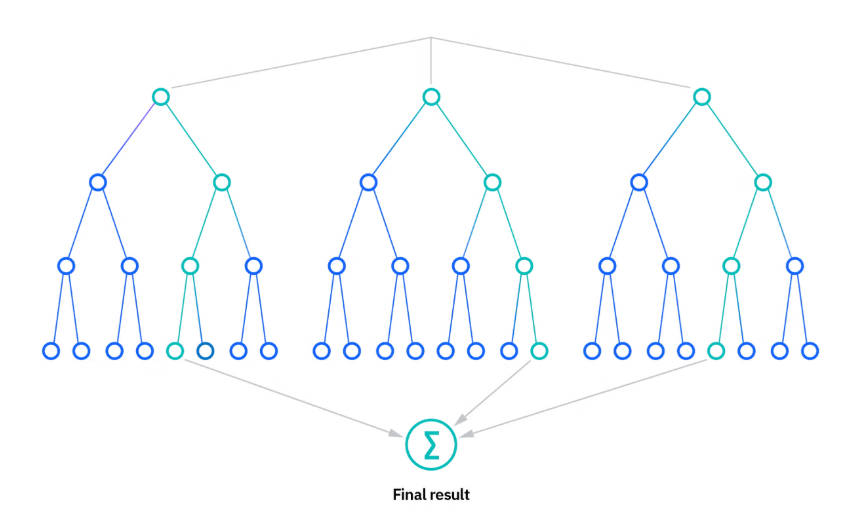
\includegraphics[width=0.7\textwidth]{Diagrams/Random Forest}
    \caption{Random Forest algorithm architecture. Source: IBM \cite{ibm_random_forest}.}
    \label{fig:random_forest}
\end{figure}

\textbf{K-Nearest Neighbors (k-NN)} is a non-parametric, supervised learning algorithm that classifies a new instance based on the classes of its nearest neighboring data points. For classification, the predicted class is determined by the majority vote among the $k$ nearest neighbors \cite{ibm_knn}. The algorithm is considered a lazy or memory-based learner because it stores the training data and performs most computations only when a prediction is made.

The distance between instances is commonly measured using Euclidean distance, expressed as

\begin{equation}
d(\mathbf{x},\mathbf{y}) =
\sqrt{\sum_{i=1}^{n}(x_i-y_i)^2},
\end{equation}

where $x_i$ and $y_i$ represent the corresponding feature values of two instances. The value of $k$ influences model behavior, where smaller values may increase variance and sensitivity to noise, while larger values may produce smoother decision boundaries with higher bias. Cross-validation can be used to determine an appropriate value of $k$ for the dataset \cite{ibm_knn}.
\begin{figure}[htbp]
    \centering
    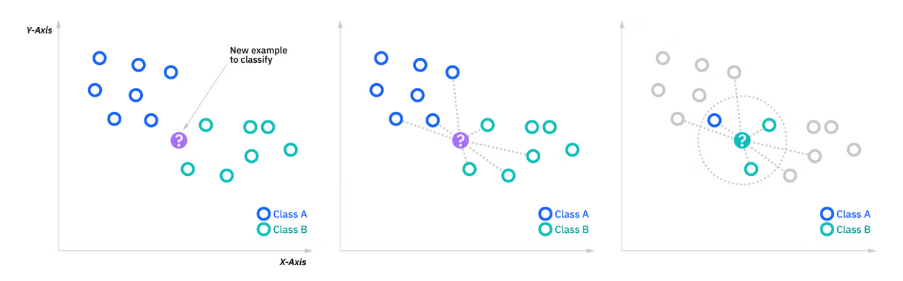
\includegraphics[width=0.7\textwidth]{Diagrams/KNN}
    \caption{Illustration of the K-Nearest Neighbors classification process. Source: IBM \cite{ibm_knn}.}
    \label{fig:knn_classification}
\end{figure}

\textbf{Gradient Boosting Machines (XGBoost, LightGBM, and CatBoost)}
are ensemble learning methods that build decision trees sequentially, where
each new tree attempts to correct errors made by the preceding trees. Through
this iterative process, the ensemble gradually improves its predictions
\cite{ibm_xgboost}.

\textbf{XGBoost (Extreme Gradient Boosting)} is an optimized implementation
of gradient-boosted decision trees that sequentially adds trees to minimize
prediction error. It incorporates regularization techniques to control model
complexity and reduce overfitting \cite{ibm_xgboost}.

\begin{figure}[H]
    \centering
    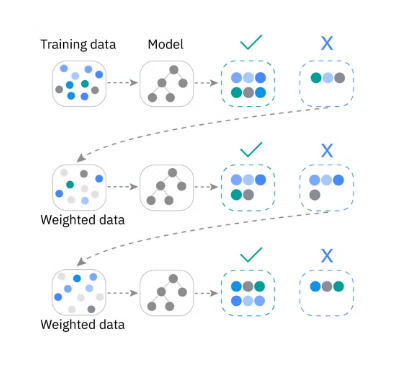
\includegraphics[width=0.75\linewidth]{Diagrams/xgboost_diagram.png}
    \caption{Sequential boosting process used in gradient-boosted decision trees.
    Source: IBM \cite{ibm_xgboost}.}
    \label{fig:xgboost}
\end{figure}

\textbf{LightGBM (Light Gradient Boosting Machine)} is a high-performance
gradient boosting framework designed for efficient training on large datasets.
Most gradient boosting implementations grow trees level-wise, splitting all
leaves at a given depth before proceeding deeper. LightGBM instead uses a
leaf-wise (best-first) strategy, where at each step the single leaf with the
greatest reduction in loss is selected for further splitting, regardless of
its depth. This produces asymmetric trees and typically achieves lower loss
than level-wise growth for the same number of iterations.
LightGBM also uses histogram-based splitting, grouping continuous feature
values into discrete bins to reduce memory usage and improve training speed
\cite{lightgbm_docs}.

\begin{figure}[H]
    \centering
    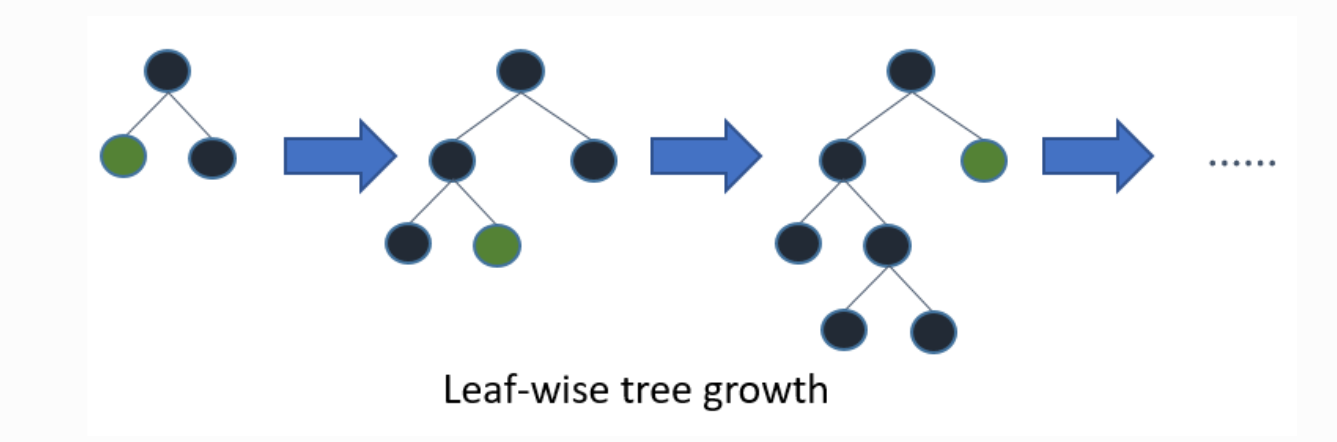
\includegraphics[width=0.75\linewidth]{Diagrams/lightgbm_diagram.png}
    \caption{Leaf-wise tree growth in LightGBM. At each step, the leaf with
    the greatest loss reduction is selected for further splitting, producing
    an asymmetric tree that grows deeper on one branch rather than expanding
    all leaves at the same depth.
    Source: LightGBM Contributors \cite{lightgbm_docs}.}
    \label{fig:lightgbm}
\end{figure}

\textbf{CatBoost (Categorical Boosting)} is a gradient boosting algorithm
designed to effectively handle both numerical and categorical features.
It can process categorical variables internally without requiring extensive
manual encoding and uses ordered boosting to help reduce overfitting
\cite{geeksforgeeks_catboost}.

\begin{figure}[H]
    \centering
    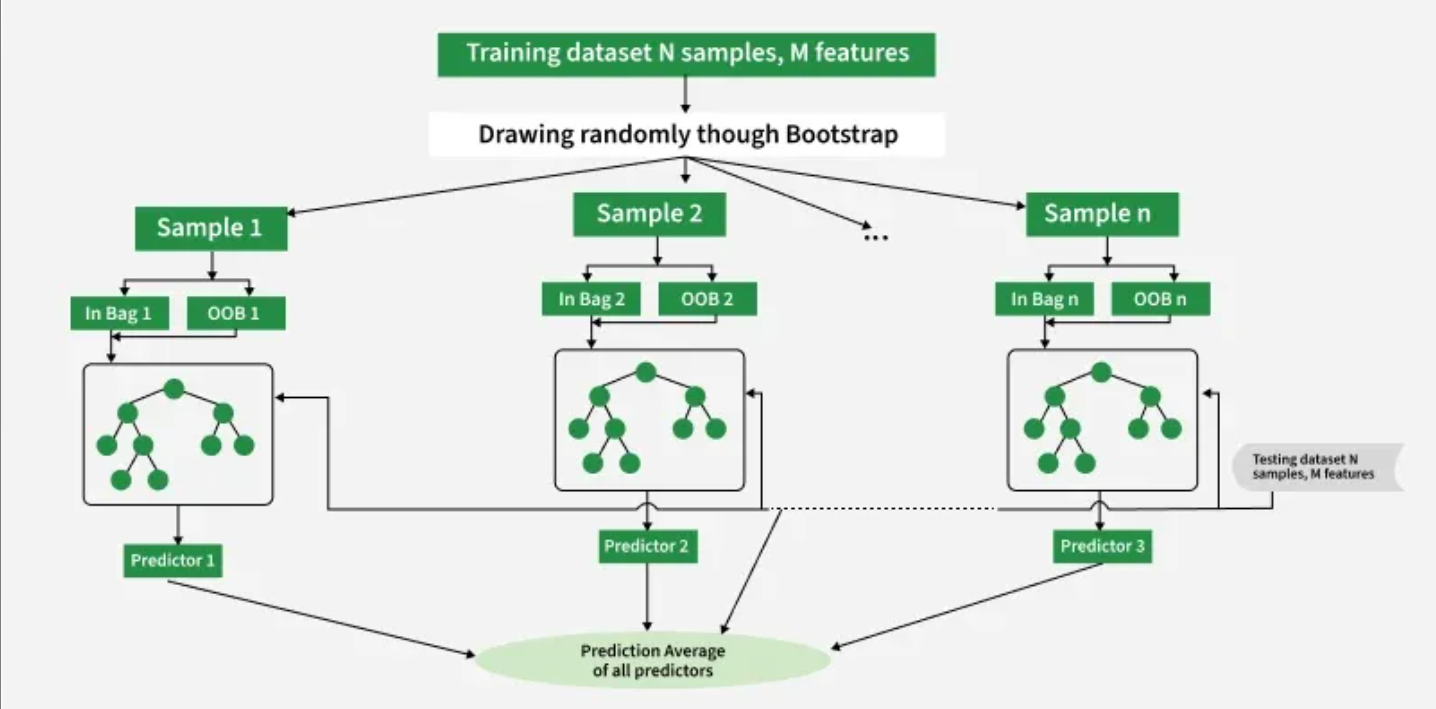
\includegraphics[width=0.75\linewidth]{Diagrams/catboost_diagram.png}
    \caption{Illustration of the CatBoost boosting process.
    Source: GeeksforGeeks \cite{geeksforgeeks_catboost}.}
    \label{fig:catboost}
\end{figure}

\subsubsection{Ensemble Learning}

Ensemble learning combines predictions from multiple trained classifiers to
produce a final output that is generally more robust than any individual
model. By aggregating outputs from models that may differ in their error
patterns, ensemble approaches can reduce prediction variability and improve
generalization performance \cite{lu_uddin_stacking_2022, gollapalli_stacking_diabetes_2022}.

This study evaluates two ensemble strategies. A \textbf{voting ensemble}
averages the predicted probabilities from a set of base classifiers and
assigns the class with the highest average probability as the final
prediction. No additional training is required after the constituent models
are fitted.

A \textbf{stacking ensemble} (stacked generalization) trains a meta-learner
on the predictions generated by a set of base models. The base models are
trained using cross-validation so that the meta-learner is fitted on
out-of-fold predictions, reducing the risk of the meta-learner overfitting
to training data. This allows the meta-learner to weight the contributions
of different base models based on their complementary strengths
\cite{lu_uddin_stacking_2022, gollapalli_stacking_diabetes_2022}.

\begin{figure}[H]
    \centering
    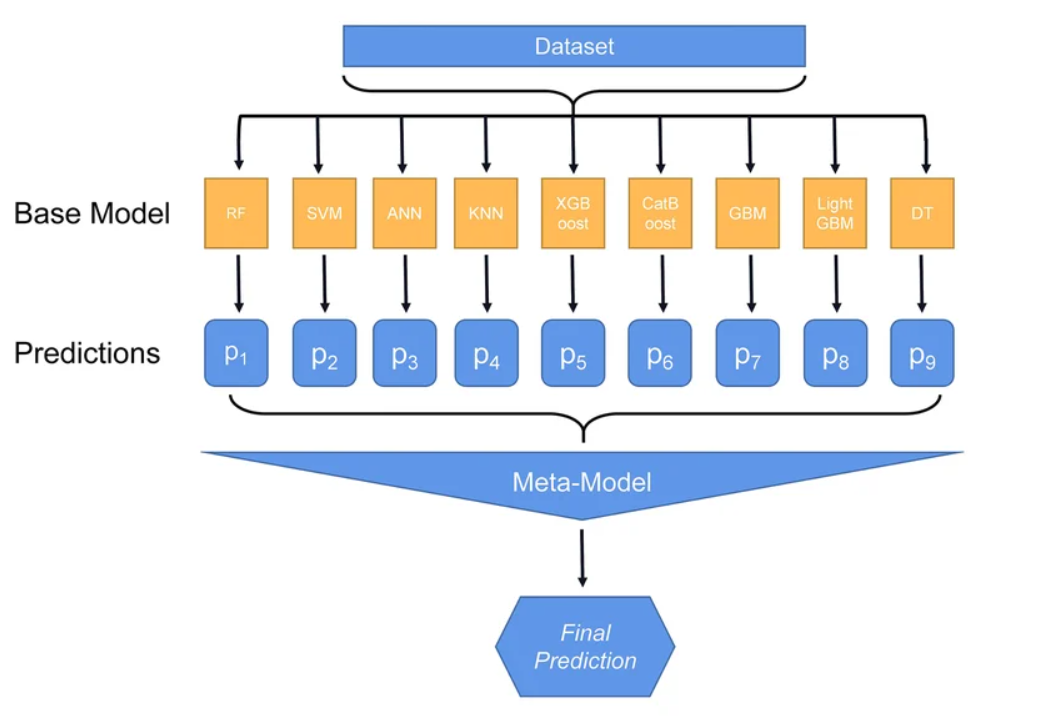
\includegraphics[width=0.75\linewidth]{Diagrams/stacking_ensemble.png}
    \caption{Illustration of the stacking ensemble learning process, showing
    base-model predictions used as inputs to a meta-learner.
    Source: Zhang et al.~\cite{zhang_stacking_2024}.}
    \label{fig:stacking}
\end{figure}

\subsubsection{Handling Class Imbalance}

\textbf{Class Imbalance} occurs when one class contains substantially fewer
instances than another, causing the learning algorithm to favor the majority
class. In medical classification, this can be problematic because a model may
achieve high overall accuracy while performing poorly in identifying the
minority class \cite{elreedy_smote_2023}.

Two complementary strategies are used in this study to address class imbalance.

\textbf{Synthetic Minority Over-sampling Technique (SMOTE)} is an oversampling
method that increases the representation of the minority class by generating
synthetic samples rather than simply duplicating existing observations.
For a selected minority instance, SMOTE identifies nearby minority-class
neighbors and generates a new sample by interpolating between them
\cite{smote_machine_failure_2023}. This approach helps provide the classifier
with a more balanced representation of both classes during training.

\begin{figure}[H]
    \centering
    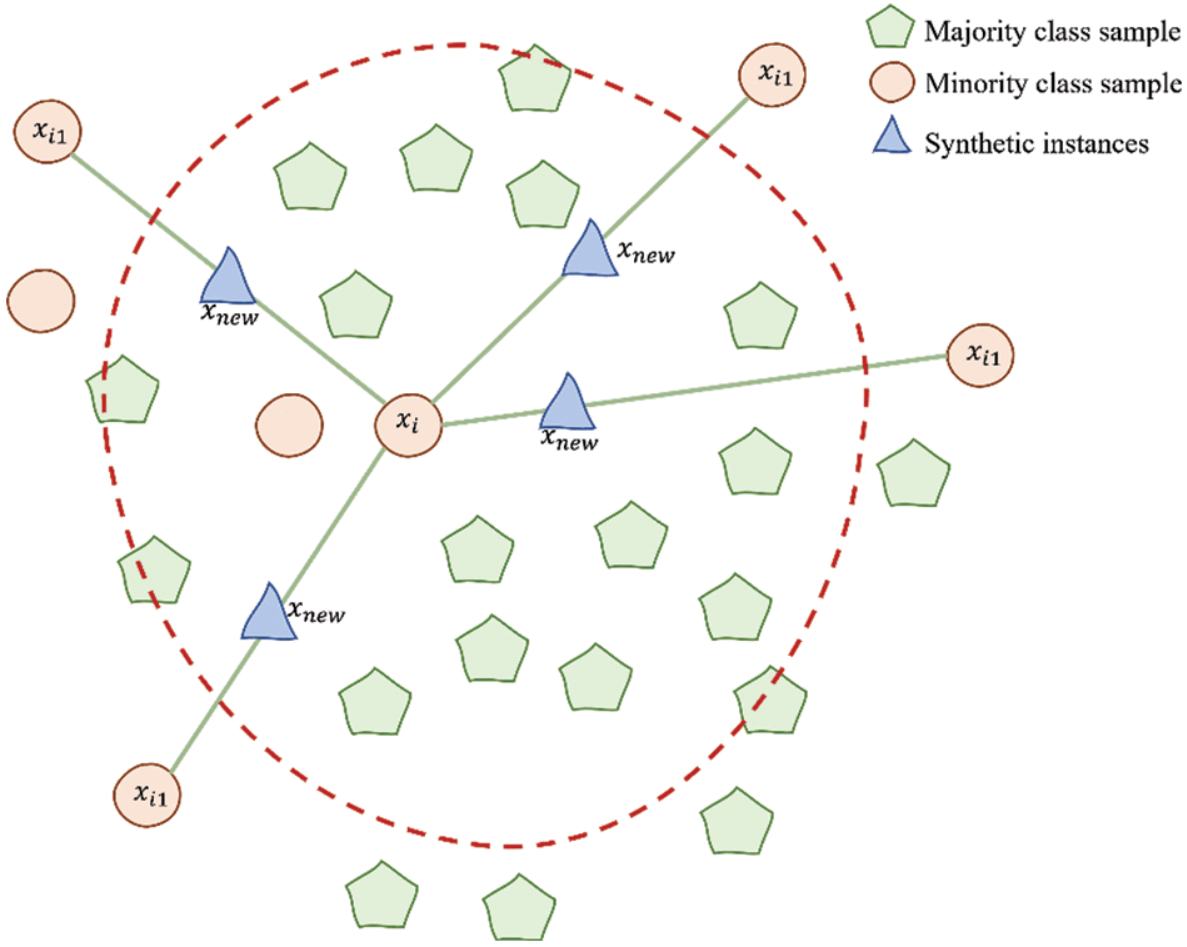
\includegraphics[width=0.70\linewidth]{Diagrams/smote_diagram.png}
    \caption{Illustration of synthetic sample generation using the SMOTE algorithm.
    Source: \cite{smote_machine_failure_2023}.}
    \label{fig:smote}
\end{figure}

A synthetic sample can be represented as

\begin{equation}
x_{\text{new}} = x_i + \lambda(x_j - x_i),
\end{equation}

where $x_i$ is a minority-class instance, $x_j$ is one of its nearest
minority-class neighbors, and $\lambda$ is a random value between 0 and 1.

\textbf{Evaluation Metric Selection} addresses class imbalance at the model
assessment stage. Because accuracy can be misleading when one class
dominates the dataset, this study uses the F2-score as the primary model
selection metric, which places greater weight on recall than precision.
The rationale and formulation for this choice are provided in the Model
Evaluation Metrics section of this framework.

\subsection{Neural Networks and Optimization Strategies}

Neural networks are computational models composed of interconnected layers
of artificial neurons. A typical architecture consists of an input layer,
one or more hidden layers, and an output layer. Each neuron computes a
weighted combination of its inputs and applies a nonlinear activation
function such as ReLU or sigmoid. During training, the network adjusts its
weights and biases to minimize a loss function and improve its predictions
\cite{ibm_neural_networks}.

\subsubsection{TabNet Architecture}

TabNet is a deep learning architecture specifically designed for tabular
data. Unlike conventional fully connected neural networks that process all
features simultaneously, TabNet uses sequential attention to select the
features that are most relevant at each decision step
\cite{arik_pfister_tabnet_2021}. The feature-selection process is
instance-wise, allowing different features to receive attention for
different observations.

\begin{figure}[H]
    \centering
    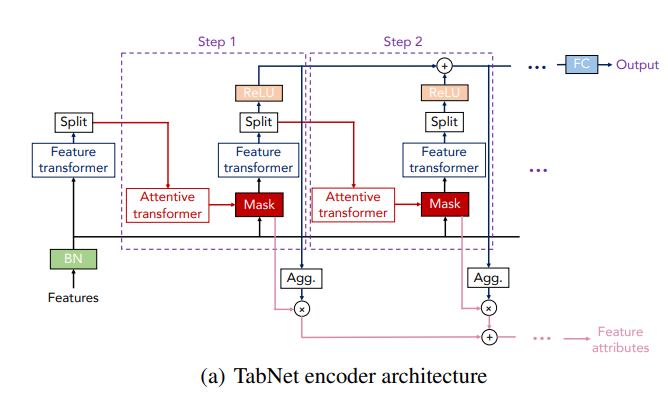
\includegraphics[width=0.90\linewidth]{Diagrams/tabnet_encoder.png}
    \caption{TabNet encoder architecture showing sequential attentive feature
    selection across decision steps. Source: Arik and Pfister
    \cite{arik_pfister_tabnet_2021}.}
    \label{fig:tabnet_encoder}
\end{figure}

The attention masks generated at each decision step also provide
interpretability by indicating which features contribute to individual
predictions. These instance-level explanations can be aggregated to obtain
global feature importance, enabling both local and global interpretation of
the model \cite{arik_pfister_tabnet_2021}. This architecture has been
applied to diabetes classification in combination with Bayesian
hyperparameter optimization and post-hoc XAI methods
\cite{joseph_tabnet_diabetes_2022}.

\subsubsection{Bayesian Optimization with Optuna}

Hyperparameters are configuration values that influence model training but
are not learned directly from the data. In TabNet, these include parameters
that control the learning process, model capacity, and regularization.
Selecting suitable hyperparameters is important because their configuration
can substantially affect predictive performance.

Bayesian Optimization is a sequential model-based approach for
hyperparameter tuning that uses information from previously evaluated
configurations to guide the selection of subsequent trials. Rather than
evaluating configurations independently, the optimization process balances
the exploration of uncertain regions of the search space with the
exploitation of configurations that are expected to perform well
\cite{bischl_hpo_2023}.

In this study, Optuna was used to optimize the hyperparameters of TabNet
over a predefined search space. Optuna's Tree-structured Parzen Estimator
(TPE) sampler models promising and less-promising regions of the search
space using separate probability distributions and selects subsequent
configurations based on their relative likelihood
\cite{optuna_tpe}. The resulting optimized architecture is referred to in
this study as BO-TabNet.

\subsection{Model Evaluation Metrics}

After the predictive models are trained and optimized, their performance
must be evaluated according to the objectives of early diabetes-risk
detection. Model evaluation determines how effectively each classifier
identifies at-risk individuals, while probability calibration subsequently
examines whether the confidence associated with those predictions is
reliable. These two aspects address different properties of predictive
performance and therefore form separate components of the proposed
framework.

\subsubsection{Precision and Recall}

Precision and Recall are fundamental evaluation metrics for binary
classification tasks, derived from the confusion matrix of true positives
(TP), true negatives (TN), false positives (FP), and false negatives (FN).

\begin{figure}[H]
    \centering
    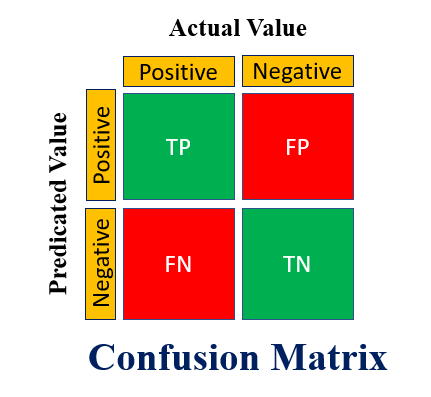
\includegraphics[width=0.62\linewidth]{Diagrams/confusion_matrix.png}
    \caption{Confusion Matrix Diagram \cite{techplayon_confusion_2025}.}

    \label{fig:confusion_matrix}
\end{figure}

Precision measures the proportion of positive predictions that are correct:

\begin{equation}
\text{Precision} = \frac{TP}{TP + FP}.
\end{equation}

Recall, also referred to as sensitivity, measures the proportion of actual
positives that are correctly identified:

\begin{equation}
\text{Recall} = \frac{TP}{TP + FN}.
\end{equation}

These two metrics often trade off against each other. In early disease
detection, recall is particularly important because failing to identify an
at-risk individual (a false negative) carries greater clinical consequence
than incorrectly flagging a not-at-risk individual (a false positive).

\subsubsection{F2-Score}

The F-beta score generalizes the F1-score by allowing the relative emphasis
placed on precision and recall to be adjusted through a parameter $\beta$:

\begin{equation}
F_\beta =
\frac{(1+\beta^2)\cdot\text{Precision}\cdot\text{Recall}}
{\beta^2\cdot\text{Precision}+\text{Recall}}.
\end{equation}

The F2-score is obtained by setting $\beta = 2$ in the generalized
$F_\beta$ measure, giving greater emphasis to recall than precision:

\begin{equation}
F_2 =
\frac{5\cdot\text{Precision}\cdot\text{Recall}}
{4\cdot\text{Precision}+\text{Recall}}.
\end{equation}

This weighting is appropriate for the study's early-risk screening
objective, where failing to identify an at-risk individual is considered
more consequential than generating an additional false-positive flag. In the
context of diabetes-risk screening, this study uses the F2-score as the
primary model selection metric.

\subsubsection{Area Under the Precision-Recall Curve}

The Precision-Recall Curve plots precision against recall as the
classification threshold varies across all possible values. The Area Under
the Precision-Recall Curve (AUPRC) summarizes this curve as a single value,
where higher values indicate stronger performance across all thresholds.

AUPRC summarizes the trade-off between precision and recall across
classification thresholds. In this study, it is particularly relevant
because evaluation focuses on the model's ability to identify the positive
at-risk class while controlling false-positive predictions. Unlike a fixed
baseline such as 0.5 for AUROC, the expected AUPRC of a random classifier
is related to the prevalence of the positive class
\cite{mcdermott_auprc_2024}.

\subsection{Probability Calibration}

Probability calibration concerns the agreement between predicted
probabilities and observed outcome frequencies. A well-calibrated model
should produce probabilities that correspond to the empirical occurrence
of the predicted outcome. For example, among individuals assigned an
approximately 70\% probability of being at risk, approximately 70\% should
belong to the at-risk class according to the study's outcome definition.

Calibration is distinct from discrimination. Discrimination describes a
model's ability to distinguish or rank positive and negative instances,
whereas calibration describes the reliability of the probabilities assigned
to those predictions. Consequently, a model may discriminate effectively
between at-risk and not-at-risk individuals while still producing poorly
calibrated probability estimates.

Calibration performance can be visualized using reliability diagrams, also known as calibration curves, which compare the mean predicted probability with the observed proportion of positive outcomes. A perfectly calibrated classifier follows the diagonal reference line, whereas deviations from this line indicate discrepancies between estimated probabilities and observed outcome frequencies. As illustrated in Figure~\ref{fig:reliability_diagram}, post-hoc calibration methods such as sigmoid calibration and isotonic regression can improve the correspondence between predicted probabilities and observed frequencies. The figure provides a conceptual example of probability calibration and does not represent the empirical results of the Philippine ENNS dataset \cite{sklearn_calibration_curves}.

\begin{figure}[H]
    \centering
    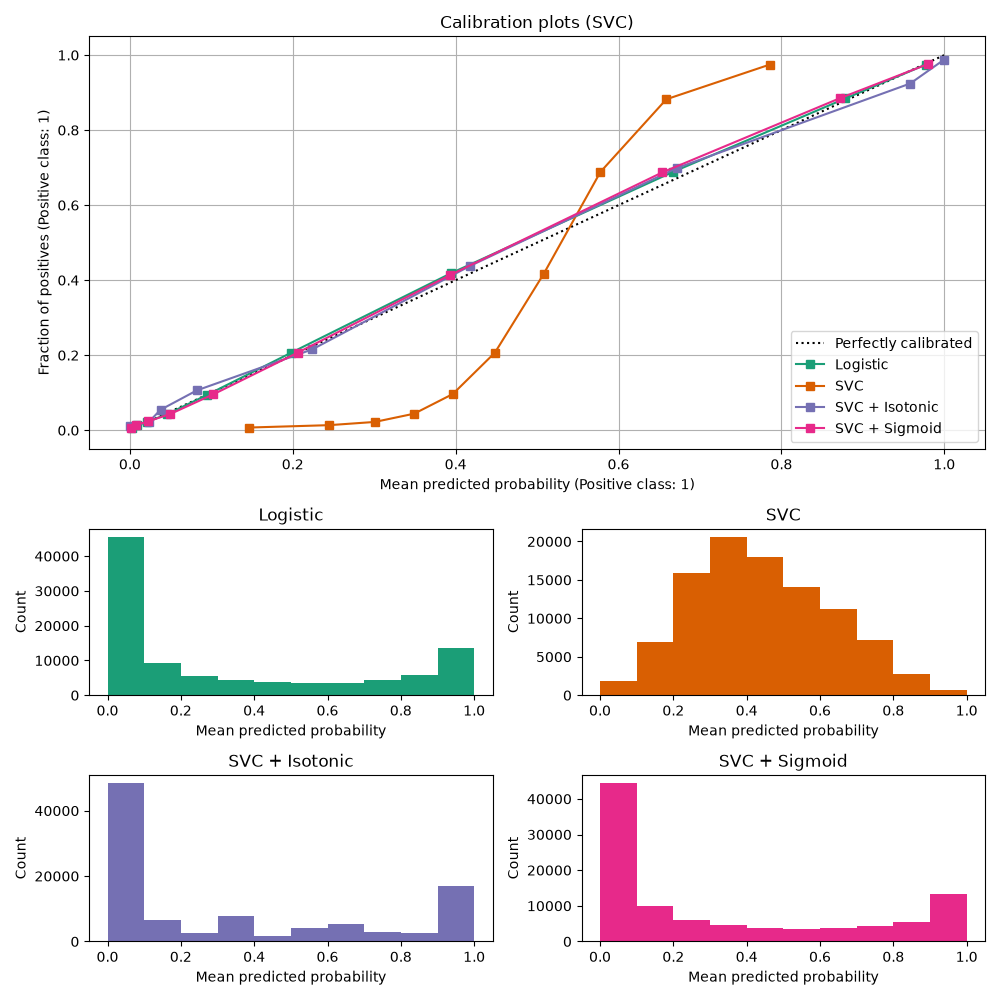
\includegraphics[width=0.72\linewidth]{Diagrams/Probability_Calibration.png}
    \caption{Reliability diagram comparing uncalibrated and calibrated model probabilities. Adapted from scikit-learn \cite{sklearn_calibration_curves}.}
    \label{fig:reliability_diagram}
\end{figure}

\subsubsection{Platt Scaling}

Platt Scaling, also known as logistic calibration, is a parametric
calibration method that maps uncalibrated model scores to calibrated
probabilities using a logistic function. Given an uncalibrated score
$f(x)$, the calibrated probability can be expressed as

\begin{equation}
P(y=1 \mid x) =
\frac{1}{1+\exp(Af(x)+B)},
\end{equation}

where $A$ and $B$ are parameters estimated using calibration data.
The logistic transformation preserves the ordering of predictions while
adjusting their probability estimates. Because it assumes a sigmoid-shaped
relationship between model scores and outcome probabilities, Platt Scaling
provides a relatively constrained parametric approach to calibration.

\subsubsection{Isotonic Regression}

Isotonic Regression is a non-parametric calibration method that learns a
monotonically increasing mapping between uncalibrated model scores and
observed outcome probabilities. Unlike Platt Scaling, it does not assume a
specific parametric form for the calibration function. Instead, it fits a
piecewise-constant function while preserving the ordering of predicted
scores.

This flexibility allows Isotonic Regression to represent more complex
calibration relationships. However, because the mapping is learned directly
from the calibration data, it can be more sensitive to limited sample sizes
than parametric approaches. In this study, Isotonic Regression provides a
flexible alternative to the parametric calibration methods.

\subsubsection{Temperature Scaling}

Temperature Scaling is a parametric post-hoc calibration method that
adjusts the confidence of a classifier by rescaling its logits using a
single positive temperature parameter $T$. For binary classification, the
calibrated probability can be expressed as

\begin{equation}
P(y=1 \mid x) =
\sigma\left(\frac{z(x)}{T}\right),
\end{equation}

where $z(x)$ represents the model logit, $T>0$ is the learned temperature
parameter, and $\sigma(\cdot)$ denotes the sigmoid function.

The temperature parameter controls the confidence of the predicted
probabilities without changing the relative ordering of the model scores.
In this study, Temperature Scaling is evaluated alongside Platt Scaling and
Isotonic Regression to determine which post-hoc calibration approach
provides the most reliable probability estimates
\cite{balanya_temperature_2024, penso_medical_calibration_2024}.

\subsubsection{Calibration Assessment}

Calibration quality can be evaluated using both graphical and quantitative
measures. Reliability diagrams compare predicted probabilities with
observed outcome frequencies, where predictions closer to the diagonal
indicate better agreement between predicted and observed probabilities.

The Brier Score measures the mean squared difference between predicted
probabilities and binary outcomes:

\begin{equation}
\mathrm{BS} =
\frac{1}{N}\sum_{i=1}^{N}(p_i-y_i)^2,
\end{equation}

where $p_i$ is the predicted probability and $y_i$ is the observed binary
outcome. Lower values indicate smaller probabilistic prediction error.

Expected Calibration Error (ECE) summarizes the discrepancy between
predicted confidence and observed positive-class frequency across
probability bins:

\begin{equation}
\mathrm{ECE} =
\sum_{m=1}^{M}
\frac{|B_m|}{N}
\left|
\mathrm{obs}(B_m)-\mathrm{conf}(B_m)
\right|,
\end{equation}

where $B_m$ represents the instances assigned to bin $m$, and
$\mathrm{obs}(B_m)$ is the observed positive-class frequency in that bin.
Lower ECE values indicate closer agreement between predicted confidence and
observed outcome frequencies.

In this study, these measures are used to compare the probability
reliability of the uncalibrated models and their Platt-scaled,
isotonic-calibrated, and temperature-scaled counterparts.

\subsection{Explainable Artificial Intelligence and Model Interpretability}

Explainable Artificial Intelligence (XAI) refers to methods that make the
behavior and predictions of machine learning models more understandable to
humans. This is particularly relevant in healthcare applications, where
predictive performance alone does not reveal which patient characteristics
influenced a model's decision \cite{xai_healthcare_review_2022}.

Model explanations can be examined from both global and local perspectives.
Global interpretation describes patterns in model behavior across the
dataset, such as the features that generally exert the greatest influence
on predictions. Local interpretation instead explains the factors
contributing to a particular individual's prediction. In this study, SHAP
and LIME are used as complementary post-hoc explanation methods for
interpreting diabetes-risk predictions.

\subsubsection{SHAP (SHapley Additive exPlanations)}

SHAP is a post-hoc explanation framework based on Shapley values from
cooperative game theory. In machine learning, the input features are treated
as contributors to a model prediction, and each feature is assigned a SHAP
value representing its contribution relative to a baseline prediction.

For feature $i$, its SHAP value can be expressed as

\begin{equation}
\phi_i =
\sum_{S \subseteq F \setminus \{i\}}
\frac{|S|!(|F|-|S|-1)!}{|F|!}
\left[
f(S \cup \{i\})-f(S)
\right],
\end{equation}

where $F$ is the complete set of features, $S$ is a subset that excludes
feature $i$, and $f(\cdot)$ represents the model output. The formulation
considers the marginal contribution of a feature across different feature
coalitions.

SHAP supports both local and global interpretation. For an individual
observation, SHAP values indicate how features contribute to its prediction.
Across multiple observations, the distribution and magnitude of SHAP values
can be aggregated to examine overall patterns of feature influence. In this study, SHAP is used to identify the features contributing to individual
diabetes-risk predictions and to examine broader patterns of model behavior
\cite{du_gdm_shap_2022, mao_diabetes_ml_2023}.

\subsubsection{LIME (Local Interpretable Model-agnostic Explanations)}

LIME is a post-hoc, model-agnostic explanation method that approximates the
behavior of a complex predictive model within the local neighborhood of an
individual observation. It generates perturbed samples around the instance
being explained, obtains predictions from the original model, and assigns
greater weight to samples that are more similar to the original observation.
A simpler interpretable surrogate model is then fitted to the weighted
samples to approximate the model's local decision behavior.

The resulting surrogate model provides an explanation of how individual
features influence the prediction within that local neighborhood. Because
the approximation is local, a LIME explanation describes the behavior of
the model around a particular observation rather than the behavior of the
model as a whole.

In this study, LIME complements SHAP by providing local surrogate-based
explanations for selected diabetes-risk predictions. Whereas SHAP assigns
feature contributions using a Shapley-value framework and can support both
local and aggregated global analysis, LIME focuses on approximating model
behavior around individual observations
\cite{wang_diabetes_lime_2023, lu_uddin_stacking_2022}.

\subsection{Calibrated Explanations and Uncertainty Quantification}

The preceding sections establish the predictive, calibration, and
explanatory foundations of the proposed framework. This section introduces
Calibrated Explanations (CE), a post-hoc framework that integrates
conformal-prediction-based calibration with feature-level interpretability.
CE addresses a limitation of conventional XAI methods such as SHAP and
LIME, which provide feature attributions without explicitly quantifying the
uncertainty associated with the underlying probability estimates
\cite{lofstrom_ce_2024}.

\subsubsection{Venn-Abers Calibration}

Venn-Abers calibration is a multi-probability calibration method derived
from Venn predictors in conformal prediction theory. Unlike standard
calibration methods that produce a single calibrated probability for each
instance, Venn-Abers calibration produces a pair of probabilities
$[p_0, p_1]$ for each prediction. These bounds represent the calibrated
probability computed under the assumption that the instance belongs to the
negative class ($p_0$) and the positive class ($p_1$), respectively.

The width of the interval $[p_0, p_1]$ reflects calibrated predictive
uncertainty: a narrow interval indicates high confidence in the calibrated
estimate, while a wider interval indicates greater uncertainty. A point
probability estimate is typically derived from the pair as a weighted
combination. Venn-Abers calibration operates under exchangeability
assumptions, and the separation between the probability bounds serves as
an indication of predictive uncertainty
\cite{nouretdinov_venn_abers_2024}.

\subsubsection{Calibrated Explanations}

Calibrated Explanations (CE) is a post-hoc, model-agnostic explanation
framework that incorporates Venn-Abers calibration into the explanation
process \cite{lofstrom_ce_2024}. For each prediction, CE produces a
calibrated probability interval alongside feature-importance scores that
include associated uncertainty ranges. This allows the explanation to
communicate not only which features contributed to a prediction but also
how reliable that prediction is.

CE is applied in this study to produce uncertainty-aware explanations for
the diabetes-risk predictions generated by the trained models. The framework
complements SHAP and LIME by integrating calibration-based uncertainty
directly into the feature attribution output, rather than treating
calibration and interpretation as separate post-processing steps.

\begin{figure}[H]
    \centering
    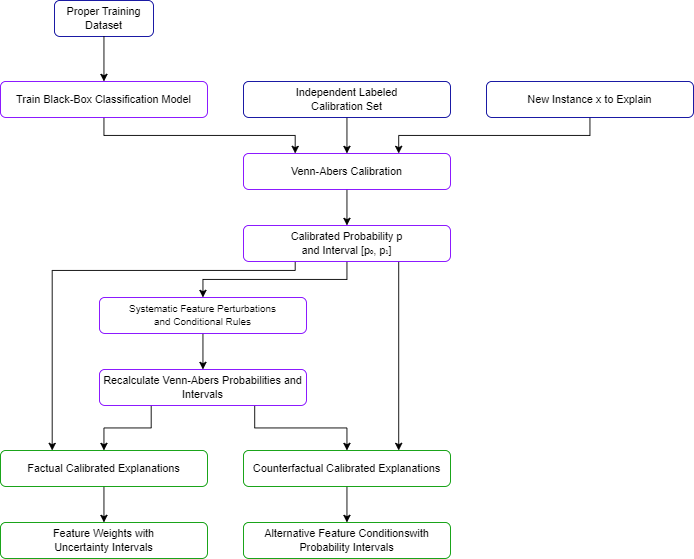
\includegraphics[width=0.92\linewidth]{Diagrams/Calibrated_Explanations_Pipeline.png}
    \caption{Conceptual flow from model prediction and Venn--Abers
    calibration to uncertainty-aware factual and counterfactual
    explanations. Authors' illustration based on
    L\"ofstr\"om et al.~\cite{lofstrom_ce_2024}.}
    \label{fig:calibrated_explanations}
\end{figure}

\subsubsection{Counterfactual Calibrated Explanations}

Counterfactual Calibrated Explanations (CCE) extend the CE framework to
generate counterfactual explanations. A counterfactual explanation
identifies feature changes or alternative conditions associated with a
change in the calibrated prediction. In the context of diabetes-risk screening, a
counterfactual explanation for an at-risk individual describes which feature
modifications would shift that individual's prediction to not at risk.

CCE incorporates Venn-Abers calibration into this process, so that the
predicted outcome associated with a counterfactual configuration is
accompanied by a calibrated probability interval rather than an
uncalibrated point estimate. This enables the counterfactual to communicate
the reliability of the hypothetical prediction alongside the feature-level
change \cite{lofstrom_ce_2024}.

\subsubsection{Mondrian Calibrated Explanations and Fairness Analysis}

Mondrian Calibrated Explanations extend the CE framework using Mondrian
conformal prediction, in which the calibration set is partitioned into
subgroups based on a conditioning variable and calibration is applied
separately within each partition. This enables group-conditional analysis
of calibration reliability and explanation consistency rather than reporting
only aggregate metrics across the entire dataset.

In this study, biological sex is used as a conditioning category to examine
whether calibrated predictions, uncertainty estimates, and explanations
behave consistently across male and female respondents. This provides a
fairness-oriented subgroup analysis without treating group-conditional
calibration alone as evidence of overall algorithmic fairness
\cite{lofstrom_conditional_ce_2024}.

Taken together, these theoretical foundations support the proposed
calibrated explainable machine learning framework for early diabetes-risk
detection. Machine learning and ensemble methods provide the predictive
foundation, while recall-sensitive evaluation addresses the clinical
importance of identifying at-risk individuals. Probability calibration
examines whether predicted risks are reliable, and SHAP and LIME provide
complementary interpretations of model behavior. Calibrated Explanations
further integrate predictive uncertainty into the explanation process, while
counterfactual and Mondrian extensions enable actionable insights and
sex-stratified analysis. Collectively, these components establish the
theoretical basis for evaluating not only whether a model predicts diabetes
risk accurately, but also whether its predictions are reliable,
interpretable, and appropriately characterized by uncertainty.

\section{Design and Implementation}

This chapter documents the operational realization of the theoretical framework presented in Chapter 3. It describes exactly how the 2018--2021 Philippine Expanded National Nutrition Survey (ENNS) data were integrated, preprocessed, and partitioned; how the ten candidate classifiers were trained and optimized; how probability calibration was applied and evaluated; and how SHAP, LIME, and Calibrated Explanations (CE) were generated. The chapter proceeds from raw data ingestion through to the full hybrid explainability pipeline, establishing the reproducible system whose results are reported in Chapter 5.

\subsection{Methodological Pipeline Overview}

The implemented pipeline follows eight sequential stages from raw ENNS data to Calibrated Explanations output: (1) multi-dataset ENNS integration; (2) ENNS sentinel-value normalization and target construction; (3) selective feature engineering; (4) missing-value imputation, outlier capping, and standardization; (5) correlation-based feature elimination producing a final 22-feature predictor set; (6) SMOTE class balancing applied to the full preprocessed dataset; (7) stratified 70/15/15 partitioning; and (8) sequential execution of model training, probability calibration, SHAP/LIME explainability, and Calibrated Explanations generation.

All data transformation parameters --- imputation statistics, outlier bounds, scaling parameters, and correlation filter decisions --- were estimated from the training partition only and applied without modification to the validation and test partitions. The ten trained classifiers span a Gaussian Na\"{i}ve Bayes baseline, six tuned traditional ML models (kNN, AdaBoost, XGBoost, Random Forest, CatBoost, LightGBM), a Bayesian-optimized deep learning model (BO-TabNet), and two ensemble architectures (Voting and Stacking). Three calibration methods (Platt Scaling, Isotonic Regression, Temperature Scaling) were applied to each model, and explanations were generated using SHAP, LIME, and the Calibrated Explanations framework with Venn-Abers calibration.

% TODO: Add Figure - end-to-end pipeline diagram
% \begin{figure}[H]
%     \centering
%     \includegraphics[width=\textwidth]{Diagrams/pipeline_overview.pdf}
%     \caption{End-to-end pipeline from 2018--2021 ENNS data ingestion to
%     Calibrated Explanations output. Authors' illustration.}
%     \label{fig:pipeline_overview}
% \end{figure}

\subsection{Data Source}

\subsubsection{2018--2021 Expanded National Nutrition Survey}

The dataset used in this study is sourced from the 2018--2021 Expanded National Nutrition Survey (ENNS), conducted by the Food and Nutrition Research Institute (FNRI) under the Department of Science and Technology (DOST) of the Philippines. The ENNS is a nationally representative survey collecting data on health, nutrition, and socioeconomic characteristics of the Filipino population across all administrative regions.

\subsubsection{ENNS Component Datasets}

Five component datasets were accessed and merged. The dietary component was examined but excluded from the final predictive feature set, as preliminary analysis indicated it introduced noise inconsistent with the study's clinical scope.

\begin{table}[H]
\centering
\caption{ENNS component datasets and their role in the final pipeline.}
\label{tab:enns_components}
\begin{tabular}{p{2.8cm}p{2cm}p{6.5cm}}
\hline
\textbf{Component} & \textbf{Status} & \textbf{Key Variables Retained} \\
\hline
Clinical/Health & Used & Ave\_SBP, Ave\_DBP, hemoglobin, uic, vita, behavioral and lifestyle variables \\
Biochemical & Used & tri, hdl, ldl \\
Anthropo\-metric & Used & waist, anthro\_group (height/weight used for feature engineering, then dropped) \\
Socioeconomic & Partial (age, sex only) & age, sex \\
Dietary & Examined; excluded & --- \\
\hline
\end{tabular}
\end{table}

The four retained component datasets were merged on the common identifiers \texttt{hhnum} (household number) and \texttt{member\_code}, using the clinical dataset as the left anchor.

\subsubsection{Diabetes Risk Target Definition}

The target variable \texttt{diabetes} was derived from fasting blood sugar (FBS). Following the American Diabetes Association diagnostic criteria \cite{ada_diabetes_diagnosis}, individuals with FBS $\geq$ 100 mg/dL (prediabetes: 100--125 mg/dL; diabetes: $\geq$126 mg/dL) were assigned Class~1 (\textit{at risk}), and those with FBS $<$ 100 mg/dL were assigned Class~0 (\textit{not at risk}). Rows with missing FBS were removed before any imputation step to prevent imputation-induced label leakage.

\subsubsection{Final Predictor Set}

Following feature engineering and correlation filtering, the final modeling set comprised 22 predictors spanning five domains.

\begin{table}[H]
\centering
\caption{Final 22-feature predictor set used in all ten classifiers.}
\label{tab:final_features}
\begin{tabular}{clll}
\hline
\textbf{\#} & \textbf{Feature} & \textbf{Type} & \textbf{Domain} \\
\hline
1 & \texttt{Ave\_SBP} & Continuous & Clinical \\
2 & \texttt{Ave\_DBP} & Continuous & Clinical \\
3 & \texttt{uic} & Continuous & Clinical \\
4 & \texttt{vita} & Continuous & Clinical \\
5 & \texttt{hemoglobin} & Continuous & Clinical \\
6 & \texttt{tri} & Continuous & Biochemical \\
7 & \texttt{hdl} & Continuous & Biochemical \\
8 & \texttt{ldl} & Continuous & Biochemical \\
9 & \texttt{waist} & Continuous & Anthropometric \\
10 & \texttt{anthro\_group} & Categorical & Demographic \\
11 & \texttt{currentsmoking} & Categorical & Behavioral \\
12 & \texttt{ever\_smk} & Categorical & Behavioral \\
13 & \texttt{smoke\_status} & Categorical & Behavioral \\
14 & \texttt{alcohol} & Categorical & Behavioral \\
15 & \texttt{con\_alcohol} & Categorical & Behavioral \\
16 & \texttt{drnk\_30days} & Categorical & Behavioral \\
17 & \texttt{drnk\_30d\_num} & Continuous & Behavioral \\
18 & \texttt{binge\_drink} & Categorical & Behavioral \\
19 & \texttt{pa\_met} & Continuous & Behavioral \\
20 & \texttt{age} & Continuous & Demographic \\
21 & \texttt{sex} & Categorical & Demographic \\
22 & \texttt{ldl\_hdl\_ratio} & Continuous & Engineered \\
\hline
\end{tabular}
\end{table}

The FBS column was removed from the feature matrix after target construction.

\subsection{Preprocessing and Feature Engineering}

All preprocessing was implemented in Python using \texttt{Pandas}, \texttt{NumPy}, \texttt{scikit-learn} (version 1.2.2), and \texttt{imbalanced-learn}. The complete pipeline is executed by \texttt{main\_preprocessing.py}.

\subsubsection{Dataset Integration}

The anthropometric, biochemical, and clinical datasets were merged via a left join on \texttt{hhnum} and \texttt{member\_code}, using the clinical dataset as the anchor. The socioeconomic dataset was subsequently merged to extract \texttt{age} and \texttt{sex}. After merging, metadata columns (\texttt{regcode}, \texttt{provhuc}, \texttt{hhnum}, \texttt{member\_code}, and survey design codes) were dropped to prevent geographic data leakage.

\subsubsection{ENNS Sentinel-Value Normalization}

The ENNS survey encodes missing, unknown, and non-applicable responses using survey-specific sentinel values (e.g., \texttt{999}, \texttt{9999}) as documented in the FNRI survey metadata. Before imputation, all such codes were recoded to \texttt{NaN} to ensure they were treated as genuine missing values.

\subsubsection{Target Construction}

Rows with missing FBS were removed before any feature imputation step, preventing imputation-induced label leakage. The binary target \texttt{diabetes} was constructed from the remaining records using the FBS threshold described in Section~4.2.3.

\subsubsection{Selective Feature Engineering}

Four candidate features were computed from raw anthropometric and biochemical measurements before imputation and scaling. Total cholesterol (\texttt{chol}) was dropped explicitly to retain the more specific LDL metric prior to correlation filtering.

\begin{table}[H]
\centering
\caption{Engineered features and their outcome after correlation filtering.}
\label{tab:engineered_features}
\begin{tabular}{p{3cm}p{3.2cm}p{1.8cm}p{4cm}}
\hline
\textbf{Feature} & \textbf{Formula} & \textbf{Status} & \textbf{Reason} \\
\hline
\texttt{bmi} & weight $\div$ (height/100)$^2$ & Dropped & $r > 0.80$ with \texttt{waist} \\
\texttt{tri\_hdl\_ratio} & tri $\div$ hdl & Dropped & $r > 0.80$ with \texttt{tri} \\
\texttt{ldl\_hdl\_ratio} & ldl $\div$ hdl & \textbf{Retained} & Adds non-redundant atherogenic signal \\
\texttt{bmi\_tri\_interact} & bmi $\times$ tri $\div$ 100 & Dropped & $r > 0.80$ with \texttt{tri} \\
\hline
\end{tabular}
\end{table}

After engineering, \texttt{weight} and \texttt{height} were dropped as they were fully captured by derived features. Only \texttt{ldl\_hdl\_ratio} survived correlation filtering as an engineered predictor.

\subsubsection{Missing-Value Imputation}

Missing values in continuous features were imputed using K-Nearest Neighbors (KNN) imputation with the number of neighbors $k$ optimized through cross-validation. Categorical features were imputed using mode values. All imputation parameters were fitted exclusively on the training partition and applied without refitting to validation and test partitions.

\subsubsection{Outlier Handling}

Outliers in continuous features were capped using the interquartile range (IQR) method with a 1.5$\times$IQR boundary. Values below $Q_1 - 1.5 \times \mathrm{IQR}$ were set to the lower bound; values above $Q_3 + 1.5 \times \mathrm{IQR}$ were set to the upper bound. IQR thresholds were computed from the training partition only.

\subsubsection{Standardization}

Continuous predictors were standardized using \texttt{StandardScaler}. The scaler was fitted on the training partition and applied without refitting to the validation and test partitions. Categorical features were left unchanged.

\subsubsection{Correlation-Based Feature Elimination}

Pearson correlation was computed across all numerical features. For each pair with $|r| > 0.80$, the feature with the lower absolute correlation with the target variable was removed iteratively. This step, together with the feature engineering filter, produced the final 22-predictor set described in Table~\ref{tab:final_features}.

\subsubsection{Class-Imbalance Handling}

The dataset exhibits class imbalance, with not-at-risk cases substantially outnumbering at-risk cases. SMOTE \cite{elreedy_smote_2023} was applied to the full preprocessed dataset with \texttt{sampling\_strategy = 1.0} (full 1:1 balance) and \texttt{k\_neighbors = 5}. The resulting balanced dataset was subsequently partitioned into training, validation, and test sets.

\subsubsection{Train-Validation-Test Partition}

The balanced dataset was partitioned using a stratified 70/15/15 split with \texttt{random\_state = 42}:

\begin{itemize}
    \item \textbf{Training set (70\%):} used for model fitting, imputation, scaling, and RandomizedSearchCV cross-validation
    \item \textbf{Validation set (15\%):} used for Optuna BO-TabNet optimization and post-hoc calibration fitting
    \item \textbf{Test set (15\%):} used exclusively for final performance evaluation; no transformation parameters were re-estimated from it
\end{itemize}

\subsection{Model Development and Optimization}

All classifiers were implemented in Python 3.9 using \texttt{scikit-learn} (version 1.2.2), \texttt{pytorch-tabnet} (version 4.0), \texttt{xgboost} (version 1.7.5), \texttt{lightgbm} (version 3.3.5), \texttt{catboost} (version 1.2), and \texttt{optuna}. Table~\ref{tab:model_optimization} summarizes the ten candidate classifiers and their optimization strategies; F2-score was the optimization objective for all tunable models.

\begin{table}[H]
\centering
\caption{Candidate classifiers and hyperparameter optimization strategy.}
\label{tab:model_optimization}
\begin{tabular}{p{3.6cm}p{4.8cm}rp{1.4cm}}
\hline
\textbf{Model} & \textbf{Optimization} & \textbf{Candidates} & \textbf{CV} \\
\hline
Na\"ive Bayes & Default (no tuning) & --- & --- \\
kNN & RandomizedSearchCV & 15 & 5-fold \\
AdaBoost & RandomizedSearchCV & 10 & 5-fold \\
XGBoost & RandomizedSearchCV & 30 & 5-fold \\
Random Forest & RandomizedSearchCV & 30 & 5-fold \\
CatBoost & RandomizedSearchCV & 30 & 5-fold \\
LightGBM & RandomizedSearchCV & 30 & 5-fold \\
BO-TabNet & Optuna/TPE & 30 trials & val set \\
Voting Ensemble & Constructed from tuned base learners & --- & --- \\
Stacking Ensemble & Logistic Regression meta-learner & --- & 5-fold \\
\hline
\end{tabular}
\end{table}

\subsubsection{RandomizedSearchCV Optimization}

For the six tunable traditional classifiers, \texttt{RandomizedSearchCV} was used with F2-score as the scoring function and 5-fold cross-validation on the training set. Representative search spaces covered: learning rate (0.01--0.3), maximum depth (3--10), and number of estimators (50--1000) for gradient-boosting models; number of neighbors and distance metric for kNN; and estimator count and learning rate for AdaBoost.

\subsubsection{Bayesian Optimization of BO-TabNet}

BO-TabNet was optimized using Optuna with the TPE sampler over 30 trials, evaluating F2-score on the validation set. The search space covered decision and attention dimensions \texttt{n\_d}/\texttt{n\_a} $\in \{8,16,32,64\}$; decision steps \texttt{n\_steps} $\in \{3,\ldots,7\}$; relaxation parameter $\gamma \in \{1.0,1.5,2.0\}$; sparsity regularization $\lambda_{\mathrm{sparse}} \in \{10^{-6},10^{-4},10^{-3}\}$; learning rate $\in \{0.005,0.01,0.02\}$; and batch size $\in \{256,512,1024\}$.

\subsubsection{Voting and Stacking Ensemble Construction}

Both ensemble classifiers used the same three optimized base learners: Random Forest, XGBoost, and LightGBM.

\textbf{Voting Ensemble:} Implemented with \texttt{VotingClassifier} (\texttt{voting=`soft'}). The final probability is the unweighted mean of the three base learners' predicted class probabilities.

\textbf{Stacking Ensemble:} Implemented with \texttt{StackingClassifier}. Out-of-fold predictions from the three base learners (via 5-fold CV) served as meta-features for a Logistic Regression meta-learner, allowing it to learn optimal weighting across the base models' complementary strengths.

\subsubsection{Model-Selection Protocol}

Models were ranked primarily by F2-score on the held-out test partition. ROC-AUC and AUPRC were retained as complementary discrimination measures, and Log-Loss and Brier Score were computed for probability quality. This dual-metric evaluation recognizes that screening performance (F2 and Recall) and deployment suitability (reliable calibrated probabilities) may favor different candidate models.

\subsection{Probability Calibration}

After training, each model's predicted probabilities are calibrated using the validation set to ensure they accurately reflect true diabetes risk. Three post-hoc calibration methods are applied and compared.

\subsubsection{Platt Scaling}

Platt Scaling fits a logistic regression model to map uncalibrated scores to calibrated probabilities. For each model, the validation set predictions are used to learn parameters $A$ and $B$ such that:

$$P_{\mathrm{calibrated}}(y=1|x) = \frac{1}{1 + \exp(A \cdot f(x) + B)}$$

where $f(x)$ is the uncalibrated score from the original model.

\subsubsection{Isotonic Regression}

Isotonic Regression fits a piecewise-constant monotonic function to map uncalibrated scores to calibrated probabilities. The calibration mapping is learned from the validation set and applied to test set predictions. Unlike Platt Scaling, Isotonic Regression does not assume a parametric form for the calibration relationship.

\subsubsection{Temperature Scaling}

Temperature Scaling adjusts model confidence by dividing the logit output by a single learned temperature parameter $T > 0$:

$$P_{\mathrm{calibrated}}(y=1|x) = \sigma\!\left(\frac{z(x)}{T}\right)$$

where $z(x)$ is the model logit and $\sigma(\cdot)$ is the sigmoid function. The temperature parameter is optimized on the validation set by minimizing negative log-likelihood. Values of $T > 1$ soften overconfident predictions, while $T < 1$ sharpens underconfident ones. Temperature Scaling does not alter the relative ranking of model predictions.

\subsubsection{Calibration Evaluation}

Calibration quality is assessed using:

\begin{itemize}
    \item \textbf{Log-Loss:} Primary calibration-selection criterion; measures the quality of predicted probability distributions
    \item \textbf{Brier Score:} Mean squared error between predicted probabilities and actual binary outcomes
    \item \textbf{ECE:} Weighted average discrepancy between predicted confidence and observed positive-class frequency across probability bins
    \item \textbf{Reliability diagrams:} Visual calibration curves comparing mean predicted probability per bin against observed positive-class frequency
\end{itemize}

For each model, the calibration method yielding the lowest Log-Loss on the test set was selected as the best calibration configuration. The best-calibrated variant of the best-discriminating model was subsequently used as the recommended deployment configuration and as the basis for the Calibrated Explanations analysis.

\subsection{Explainable Artificial Intelligence Techniques}

Three complementary XAI frameworks are implemented to provide interpretable explanations for model predictions at both global and local levels.

\subsubsection{SHAP (SHapley Additive exPlanations)}

SHAP is implemented using the SHAP Python library. For tree-based models (Random Forest, XGBoost, LightGBM, CatBoost), TreeExplainer computes exact Shapley values efficiently. For other models, KernelExplainer approximates Shapley values through sampling.

SHAP provides:
\begin{itemize}
    \item \textbf{Global Feature Importance:} Ranking of features by mean absolute SHAP value across all instances
    \item \textbf{Local Explanations:} Feature contributions for individual predictions shown through force plots and waterfall charts
    \item \textbf{Summary Plots:} Distribution of SHAP values across all instances, revealing feature impact patterns
\end{itemize}

\subsubsection{LIME (Local Interpretable Model-agnostic Explanations)}

LIME is implemented using the \texttt{lime} Python library. For each instance to be explained, LIME generates perturbed samples in the neighborhood of the observation, obtains predictions from the original model for each perturbed sample, and fits a weighted linear regression surrogate model to approximate local model behavior. Samples closer to the original instance receive higher weights in the fitting process.

LIME provides local explanations that identify which features most influenced the prediction for a specific individual, complementing the global and aggregated perspective of SHAP with a locally faithful approximation of model decision behavior.


\subsection{Evaluation Metrics}

Model performance was evaluated on the held-out test partition using seven classification metrics and four calibration metrics. Mathematical definitions are provided in Chapter~3. Table~\ref{tab:metrics_roles} documents the role of each metric in this study.

\begin{table}[H]
\centering
\caption{Evaluation metrics and their roles in this study.}
\label{tab:metrics_roles}
\begin{tabular}{p{3.3cm}p{6.8cm}l}
\hline
\textbf{Metric} & \textbf{Purpose} & \textbf{Priority} \\
\hline
\multicolumn{3}{l}{\textit{Classification Performance}} \\
F2-Score & Recall-weighted metric; primary model-selection criterion & Primary \\
Recall & Proportion of at-risk cases correctly identified & Primary \\
Precision & Positive predictive value & Supplementary \\
F1-Score & Balanced harmonic mean of Precision and Recall & Supplementary \\
ROC-AUC & Overall discrimination across all classification thresholds & Supplementary \\
AUPRC & Discrimination focused on the positive at-risk class & Supplementary \\
Accuracy & Overall correctness (limited value under class imbalance) & Supplementary \\
\hline
\multicolumn{3}{l}{\textit{Calibration Quality}} \\
Log-Loss & Primary calibration-selection criterion & Primary \\
Brier Score & Mean squared probability error & Supplementary \\
ECE & Bin-weighted confidence--frequency discrepancy & Supplementary \\
Reliability diagram & Visual calibration curve per model & Supplementary \\
\hline
\end{tabular}
\end{table}

F2-score was used as the primary classification metric because the study prioritizes sensitivity to at-risk respondents; a missed diagnosis carries greater clinical cost than a false alarm in a diabetes-screening context. Log-Loss was used as the primary calibration-selection metric to identify the best-performing calibration configuration per model.

\subsection{Calibrated Explanations Implementation}

\subsubsection{Scope and Model Coverage}

Calibrated Explanations (CE) were implemented using the \texttt{calibrated-explanations} Python library \cite{lofstrom_ce_2024}. CE was applied to nine of the ten trained classifiers; BO-TabNet was excluded because its \texttt{pytorch-tabnet} interface is incompatible with the scikit-learn estimator contract required by the CE framework.

For each compatible model, the validation partition was supplied to the CE framework as the calibration dataset for fitting internal Venn-Abers calibration. Test instances were used for generating individual and aggregated explanations. The four CE experiment types are described below.

\subsubsection{Factual Calibrated Explanations}

Factual CE was generated for six test instances per model: three predicted as at risk and three predicted as not at risk. Each explanation reports a Venn-Abers calibrated probability interval $[p_0, p_1]$ alongside per-feature importance scores with associated uncertainty ranges. Outputs are stored in \texttt{MAIN\_CE\_OUTPUT/factual/}.

\subsubsection{Counterfactual CE and Ensured CCE}

Counterfactual CE (CCE) and Ensured CCE were generated for the same six test instances per model. Ordinary CCE identifies feature changes associated with a shift in the calibrated predicted class. Ensured CCE additionally constrains the alternative prediction to carry a calibrated probability above a defined confidence threshold, ensuring the counterfactual outcome is reliably supported. Six explanation plots per model are stored in \texttt{MAIN\_CE\_OUTPUT/counterfactual/}.

\subsubsection{Global CE Aggregation}

Global CE was computed across 150 test instances per model for all nine CE-compatible classifiers. Per-instance CE feature weights were aggregated to yield a model-level mean feature importance; the standard deviation of feature weight bounds was computed as the uncertainty width --- a measure of how consistently a feature drives predictions across patients. This uncertainty width complements the SHAP global ranking by quantifying per-feature explanation stability. Outputs are stored in \texttt{MAIN\_CE\_OUTPUT/global/}.

\subsubsection{Mondrian CE for Sex-Stratified Analysis}

Mondrian CE was applied to 50 test instances per sex group per model across the nine CE-compatible classifiers. The validation set was partitioned by the \texttt{sex} variable into two groups, and Venn-Abers calibration was fitted separately within each group. This produces group-conditional calibrated explanations, enabling examination of whether prediction uncertainty and feature attribution patterns are consistent across both sex groups \cite{lofstrom_conditional_ce_2024}. Outputs are stored in \texttt{MAIN\_CE\_OUTPUT/mondrian/}.

\subsection{Reproducibility and Implementation Environment}

\subsubsection{Pipeline Scripts}

The complete pipeline is organized into eight scripts executed sequentially:

\begin{table}[H]
\centering
\caption{Pipeline scripts and their functions.}
\label{tab:scripts}
\begin{tabular}{p{4.8cm}p{7.5cm}}
\hline
\textbf{Script} & \textbf{Function} \\
\hline
\texttt{main\_preprocessing.py} & Data integration, sentinel-value normalization, target construction, feature engineering, imputation, outlier capping, standardization, correlation filtering, SMOTE, and partitioning \\
\texttt{main\_train.py} & Model training and hyperparameter optimization (10 classifiers) \\
\texttt{main\_xai.py} & SHAP and LIME explainability \\
\texttt{main\_calibration.py} & Post-hoc probability calibration (3 methods) \\
\texttt{ce\_factual.py} & Factual Calibrated Explanations (9 models) \\
\texttt{ce\_cce.py} & Counterfactual CE and Ensured CCE (9 models) \\
\texttt{ce\_global.py} & Global CE aggregation across 150 test instances \\
\texttt{ce\_mondrian.py} & Mondrian CE for sex-stratified analysis \\
\hline
\end{tabular}
\end{table}

\subsubsection{Reproducibility Settings}

All stochastic operations used \texttt{random\_state = 42}. Trained model artifacts and preprocessing transformers are persisted using \texttt{joblib} in \texttt{MAIN\_TRAINED\_MODELS/} and \texttt{MAIN\_PREPROCESS\_OUTPUT/}, respectively. Calibration objects are stored in \texttt{MAIN\_CALIBRATION/}. CE outputs are organized under \texttt{MAIN\_CE\_OUTPUT/} in subdirectories \texttt{factual/}, \texttt{counterfactual/}, \texttt{global/}, and \texttt{mondrian/}.

\section{Expected Output/Timeline}

\subsection{Project Development Timeline}

The proposed development of DiaScope AI is organized into five phases over a 26-week period. These phases cover data acquisition and preprocessing, model development and optimization, explainability and calibration integration, web application development, and system testing and documentation. Table~\ref{tab:timeline} summarizes the planned activities and their durations, while Figure~\ref{fig:project_gantt} illustrates the corresponding development schedule.

\begin{table}[H]
\centering
\caption{Proposed project development timeline.}
\label{tab:timeline}
\begin{tabular}{p{2.5cm}p{4.2cm}p{3.2cm}p{2.1cm}p{1.2cm}}
\hline
\textbf{Phase} & \textbf{Main Activities} & \textbf{Expected Output} & \textbf{Status} & \textbf{Duration} \\
\hline
1. Dataset acquisition and preprocessing & ENNS integration, target construction, feature engineering, imputation, scaling, SMOTE, and partitioning & Preprocessed datasets and saved preprocessing objects & Completed in V2 & 1-4 weeks \\
2. Model development and optimization & Training and tuning of ten classification approaches & Trained models and performance results & Completed in V2 & 5-14 weeks \\
3. XAI, calibration, and CE integration & SHAP, LIME, probability calibration, and CE analyses & Explanation outputs and calibration comparison & Completed in V2 & 15-17 weeks \\
4. Web application design and implementation & Interface design, framework selection, and integration of saved artifacts & Working prototype of the application & Not yet started & 18-23 weeks \\
5. Integration testing, evaluation, and documentation & Testing of input handling and outputs, and thesis writing & Tested prototype and final manuscript & In progress (documentation) & 24-26 weeks \\
\hline
\end{tabular}
\end{table}

\begin{figure}[H]
    \centering
    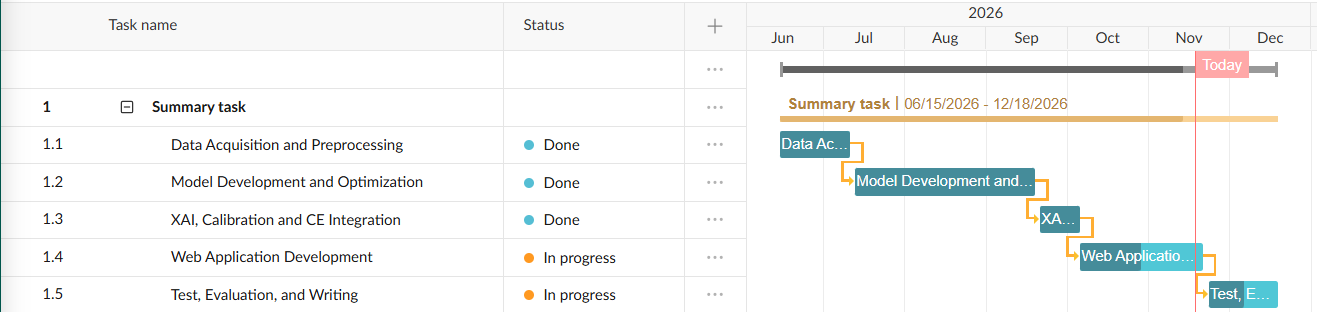
\includegraphics[width=0.95\textwidth]{Diagrams/Gantt_Chart.png}
    \caption{Proposed development schedule for the diabetes risk assessment system. Authors' illustration.}
    \label{fig:project_gantt}
\end{figure}

\subsection{User Interface Design}

The interface designs below represent how users are expected to interact with the proposed system. They are proposed layouts and are not screenshots of an implemented application.

\subsubsection{Landing Page}

The proposed landing page will present the application title and a brief description of the diabetes risk assessment system. It will state that the application is an exploratory decision-support tool and that its results do not replace professional medical evaluation. A single main control will allow the user to begin an assessment.

% PROPOSAL FIGURE PLACEHOLDER: Create Diagrams/landing_page_mockup.pdf before uncommenting.
% \begin{figure}[H]
%     \centering
%     \includegraphics[width=0.9\textwidth]{Diagrams/landing_page_mockup.pdf}
%     \caption{Proposed landing page of the diabetes risk assessment application. Authors' illustration.}
%     \label{fig:landing_page_mockup}
% \end{figure}

\subsubsection{Health Information Input Interface}

The proposed input form will follow the 22-predictor schema in Table~\ref{tab:final_features}. Fields will be grouped into demographic information, anthropometric measurements, clinical and biochemical measurements, and lifestyle and behavioral information. Each quantitative field will show its unit, required fields will be marked, and values will be validated before submission. The form will also offer a CSV upload option. Derived predictors such as \texttt{ldl\_hdl\_ratio} will be computed by the system and not entered by the user. Whether generated variables such as \texttt{smoke\_status} and \texttt{anthro\_group} can be derived from other inputs remains to be determined. Fasting blood sugar will not be requested because it defines the target label, and dietary fields will not be included because dietary predictors were excluded from the final V2 model.

% PROPOSAL FIGURE PLACEHOLDER: Create Diagrams/health_input_mockup.pdf before uncommenting.
% \begin{figure}[H]
%     \centering
%     \includegraphics[width=0.9\textwidth]{Diagrams/health_input_mockup.pdf}
%     \caption{Proposed health information input interface for diabetes risk assessment. Authors' illustration.}
%     \label{fig:health_input_mockup}
% \end{figure}

\subsubsection{Risk Assessment and Explanation Dashboard}

The proposed dashboard will contain four information areas. The risk assessment summary will show the predicted elevated-FBS risk classification, the calibrated probability, and a brief interpretation. Chapter~1 describes Low, Moderate, and High risk levels, and the probability cut-offs for these levels were not defined in the V2 experiments and will be specified during application design. The SHAP and LIME area will show the factors influencing the prediction as a local explanation. The Calibrated Explanations area will show the CE factual explanation, the Venn-Abers probability uncertainty interval, and the uncertainty of the feature weights.

The counterfactual area will show alternative feature conditions together with their estimated effect on the calibrated probability. These scenarios will be labeled as hypothetical changes in model predictions and not as guaranteed clinical interventions. Mondrian CE is a group-level evaluation and will not be shown as an individual fairness score. Only information that is understandable to the intended user will be displayed, and not every research visualization will be included.

% PROPOSAL FIGURE PLACEHOLDER: Create Diagrams/results_dashboard_mockup.pdf before uncommenting.
% \begin{figure}[H]
%     \centering
%     \includegraphics[width=0.95\textwidth]{Diagrams/results_dashboard_mockup.pdf}
%     \caption{Proposed risk assessment and explanation dashboard. Authors' illustration.}
%     \label{fig:results_dashboard_mockup}
% \end{figure}

\addcontentsline{toc}{section}{References}
\bibliographystyle{ieeetr}
\bibliography{biblio}

\end{document}


